\documentclass[a4paper,11pt,parskip=half,numbers=noenddot]{scrreprt}

% --- Language & fonts ---
\usepackage[ngerman]{babel}
\usepackage[utf8]{inputenc}
\usepackage[T1]{fontenc}
\usepackage{csquotes}
\usepackage{xparse}

% Frankfurt UAS house style (docx original): headings/title in Cambria,
% body text in Calibri -- reproduced with the metric-compatible free
% substitutes Caladea/Carlito.
\usepackage[default]{carlito}
\usepackage{caladea}

% --- Page layout ---
\usepackage[a4paper,margin=2.5cm,headheight=36pt]{geometry}
\usepackage{setspace}
\onehalfspacing

% --- Graphics & floats ---
\usepackage{graphicx}
\usepackage{float}
% Float-Platzierung lockern, damit Bilder nicht ans Dokumentende abgedrängt
% werden: mehr Bilder pro Seite erlauben, mehr Textanteil pro Seite fürs
% Ausweichen auf Floats zulassen.
\renewcommand{\topfraction}{0.9}
\renewcommand{\bottomfraction}{0.8}
\renewcommand{\textfraction}{0.1}
\renewcommand{\floatpagefraction}{0.75}
\setcounter{topnumber}{3}
\setcounter{bottomnumber}{2}
\setcounter{totalnumber}{5}
% Floats nie über eine \section-Grenze hinaus verschieben, damit sie in der
% Nähe der Textstelle bleiben, an der sie referenziert werden.
\usepackage[section]{placeins}
\usepackage{caption}
\captionsetup{font=small,labelfont=bf,labelsep=colon}
% Arbeitshilfen-Vorgabe: Bezeichnung "Bild N: Titel (Quelle)", fettgedruckt
% babel(ngerman) reasserts \figurename/\listfigurename at \begin{document},
% so the override must live in \captionsngerman, not a plain \renewcommand.
\addto\captionsngerman{%
  \renewcommand{\figurename}{Bild}%
  \renewcommand{\listfigurename}{Bildverzeichnis}%
}
\usepackage{booktabs}
\usepackage{longtable}
\usepackage{array}
\usepackage{enumitem}
\usepackage{siunitx}
\sisetup{output-decimal-marker={,},group-separator={.}}

% --- Math ---
\usepackage{amsmath}
\usepackage{amssymb}

% --- Colors (Hochschul-Farbschema, aus dem Original-Deckblatt/Vorlagenthema) ---
\usepackage[table]{xcolor}
\definecolor{unidark}{HTML}{17365D}
\definecolor{unimid}{HTML}{365F91}
\definecolor{uniaccent}{HTML}{4F81BD}

% --- Heading style (Farbe/Schnitt wie im Original-Word-Thema) ---
\usepackage{titlesec}
\titleformat{\chapter}[hang]
  {\normalfont\Huge\bfseries\color{unidark}}{\thechapter}{1em}{}
% KOMA-Script schiebt \chapter sonst immer auf eine neue Seite
% (\scr@startchapter enthält ein eingebautes \clearpage). Das entfernt
% unnötige Leerräume/Seiten am Kapitelende, indem Kapitel wie Abschnitte
% direkt im Textfluss weiterlaufen.
\usepackage{etoolbox}
\makeatletter
\patchcmd{\scr@startchapter}{\if@openright\cleardoublepage\else\clearpage\fi}{}{}{%
  \ClassWarning{scrreprt}{Could not remove automatic page break before \string\chapter}%
}
\makeatother
\titleformat{\section}
  {\normalfont\Large\bfseries\color{unimid}}{\thesection}{1em}{}
\titleformat{\subsection}
  {\normalfont\large\bfseries\color{unimid}}{\thesubsection}{1em}{}
\titleformat{\subsubsection}
  {\normalfont\normalsize\bfseries\color{unimid}}{\thesubsubsection}{1em}{}

% --- Header / Footer (Logos wie im Original-Deckblatt) ---
\usepackage{fancyhdr}
\pagestyle{fancy}
\fancyhf{}
\fancyhead[L]{
\includegraphics[height=0.75cm]{logos/UIREKA_logo_trim.png}}
\fancyhead[R]{
\includegraphics[height=0.75cm]{logos/FUAS_logo_trim.jpg}}
\fancyfoot[L]{\small\color{unimid}\Kurztitel}
\fancyfoot[R]{\small\color{unimid}\thepage}
\renewcommand{\headrulewidth}{0.4pt}
\renewcommand{\headrule}{\hbox to\headwidth{\color{uniaccent}\leaders\hrule height\headrulewidth\hfill}}
\renewcommand{\footrulewidth}{0pt}

\fancypagestyle{plain}{%
  \fancyhf{}
  \fancyhead[L]{
\includegraphics[height=0.75cm]{logos/UIREKA_logo_trim.png}}
  \fancyhead[R]{
\includegraphics[height=0.75cm]{logos/FUAS_logo_trim.jpg}}
  \fancyfoot[L]{\small\color{unimid}\Kurztitel}
  \fancyfoot[R]{\small\color{unimid}\thepage}
  \renewcommand{\headrulewidth}{0.4pt}
  \renewcommand{\headrule}{\hbox to\headwidth{\color{uniaccent}\leaders\hrule height\headrulewidth\hfill}}
  \renewcommand{\footrulewidth}{0pt}
}

\newcommand{\Kurztitel}{Radlogistik Havixbeck}

% --- Links ---
\usepackage{hyperref}
\usepackage{xurl} % allows breaking long URLs at any character, avoiding the stretched inter-word spaces that unbreakable URLs cause in justified bibliography text
\usepackage{bookmark}
\emergencystretch=3em % extra give for justification so long unbreakable DOI/URL tokens don't overflow into the margin

% --- Bibliography (author-year, close to APA style used in the original) ---
\usepackage[
  backend=biber,
  style=authoryear,
  dashed=false,
  maxcitenames=2,
  maxbibnames=99,
  uniquename=false,
  uniquelist=false,
  giveninits=true,
  sorting=nyt
]{biblatex}
\addbibresource{references.bib}
\DefineBibliographyStrings{ngerman}{andothers={et al\adddot}}

\hypersetup{
  colorlinks=true,
  linkcolor=unimid,
  citecolor=unimid,
  urlcolor=unimid,
  pdftitle={Betriebliche Kurzstrecken und die lokale B2B-Logistik in Havixbeck},
  pdfauthor={Kana Mohammad, Urs Eble, Miguel Ureña Pliego}
}

\newcommand{\vgl}[1]{(vgl.\ \citeauthor{#1} \citeyear{#1})}
% Kurzverweis für Bildunterschriften, deren Kartendarstellung auf den
% berechneten Routen der eigenen Routing-Engine beruht und daher auch in
% der interaktiven Karte einsehbar ist. Optionales Layer-Label + Query-String
% verlinken direkt auf die passende Ansicht (?layer=... / ?raster=...) statt
% immer auf die Standardansicht der Karte.
\NewDocumentCommand{\interaktivekarte}{o o}{%
  , interaktive Version\IfValueT{#1}{ (Layer \glqq#1\grqq)}%
  \ unter \url{https://miguelurenapliego.github.io/RadlogistikHavixbeck/loop_map.html\IfValueT{#2}{?#2}}%
}

\begin{document}

% ============================================================
% TITLE PAGE
% ============================================================
\begin{titlepage}
\thispagestyle{empty}
\noindent
\begin{minipage}[c][2.2cm][c]{0.48\textwidth}

\includegraphics[height=1.5cm]{logos/UIREKA_logo_trim.png}
\end{minipage}%
\hfill
\begin{minipage}[c][2.2cm][c]{0.48\textwidth}
\raggedleft

\includegraphics[height=1.9cm]{logos/FUAS_logo_trim.jpg}
\end{minipage}

\vspace{0.7cm}

\begin{center}
{\Huge\bfseries\color{unidark}\rmfamily Radlogistik\par}
\vspace{0.25cm}
\textcolor{uniaccent}{\rule{0.6\textwidth}{1pt}}
\vspace{0.4cm}

{\Large\color{unimid}\bfseries Betriebliche Kurzstrecken und die lokale\\
B2B-Logistik in Havixbeck, Kreis Coesfeld,\\
Nordrhein-Westfalen\par}
\end{center}

\vspace{0.6cm}

\begin{center}
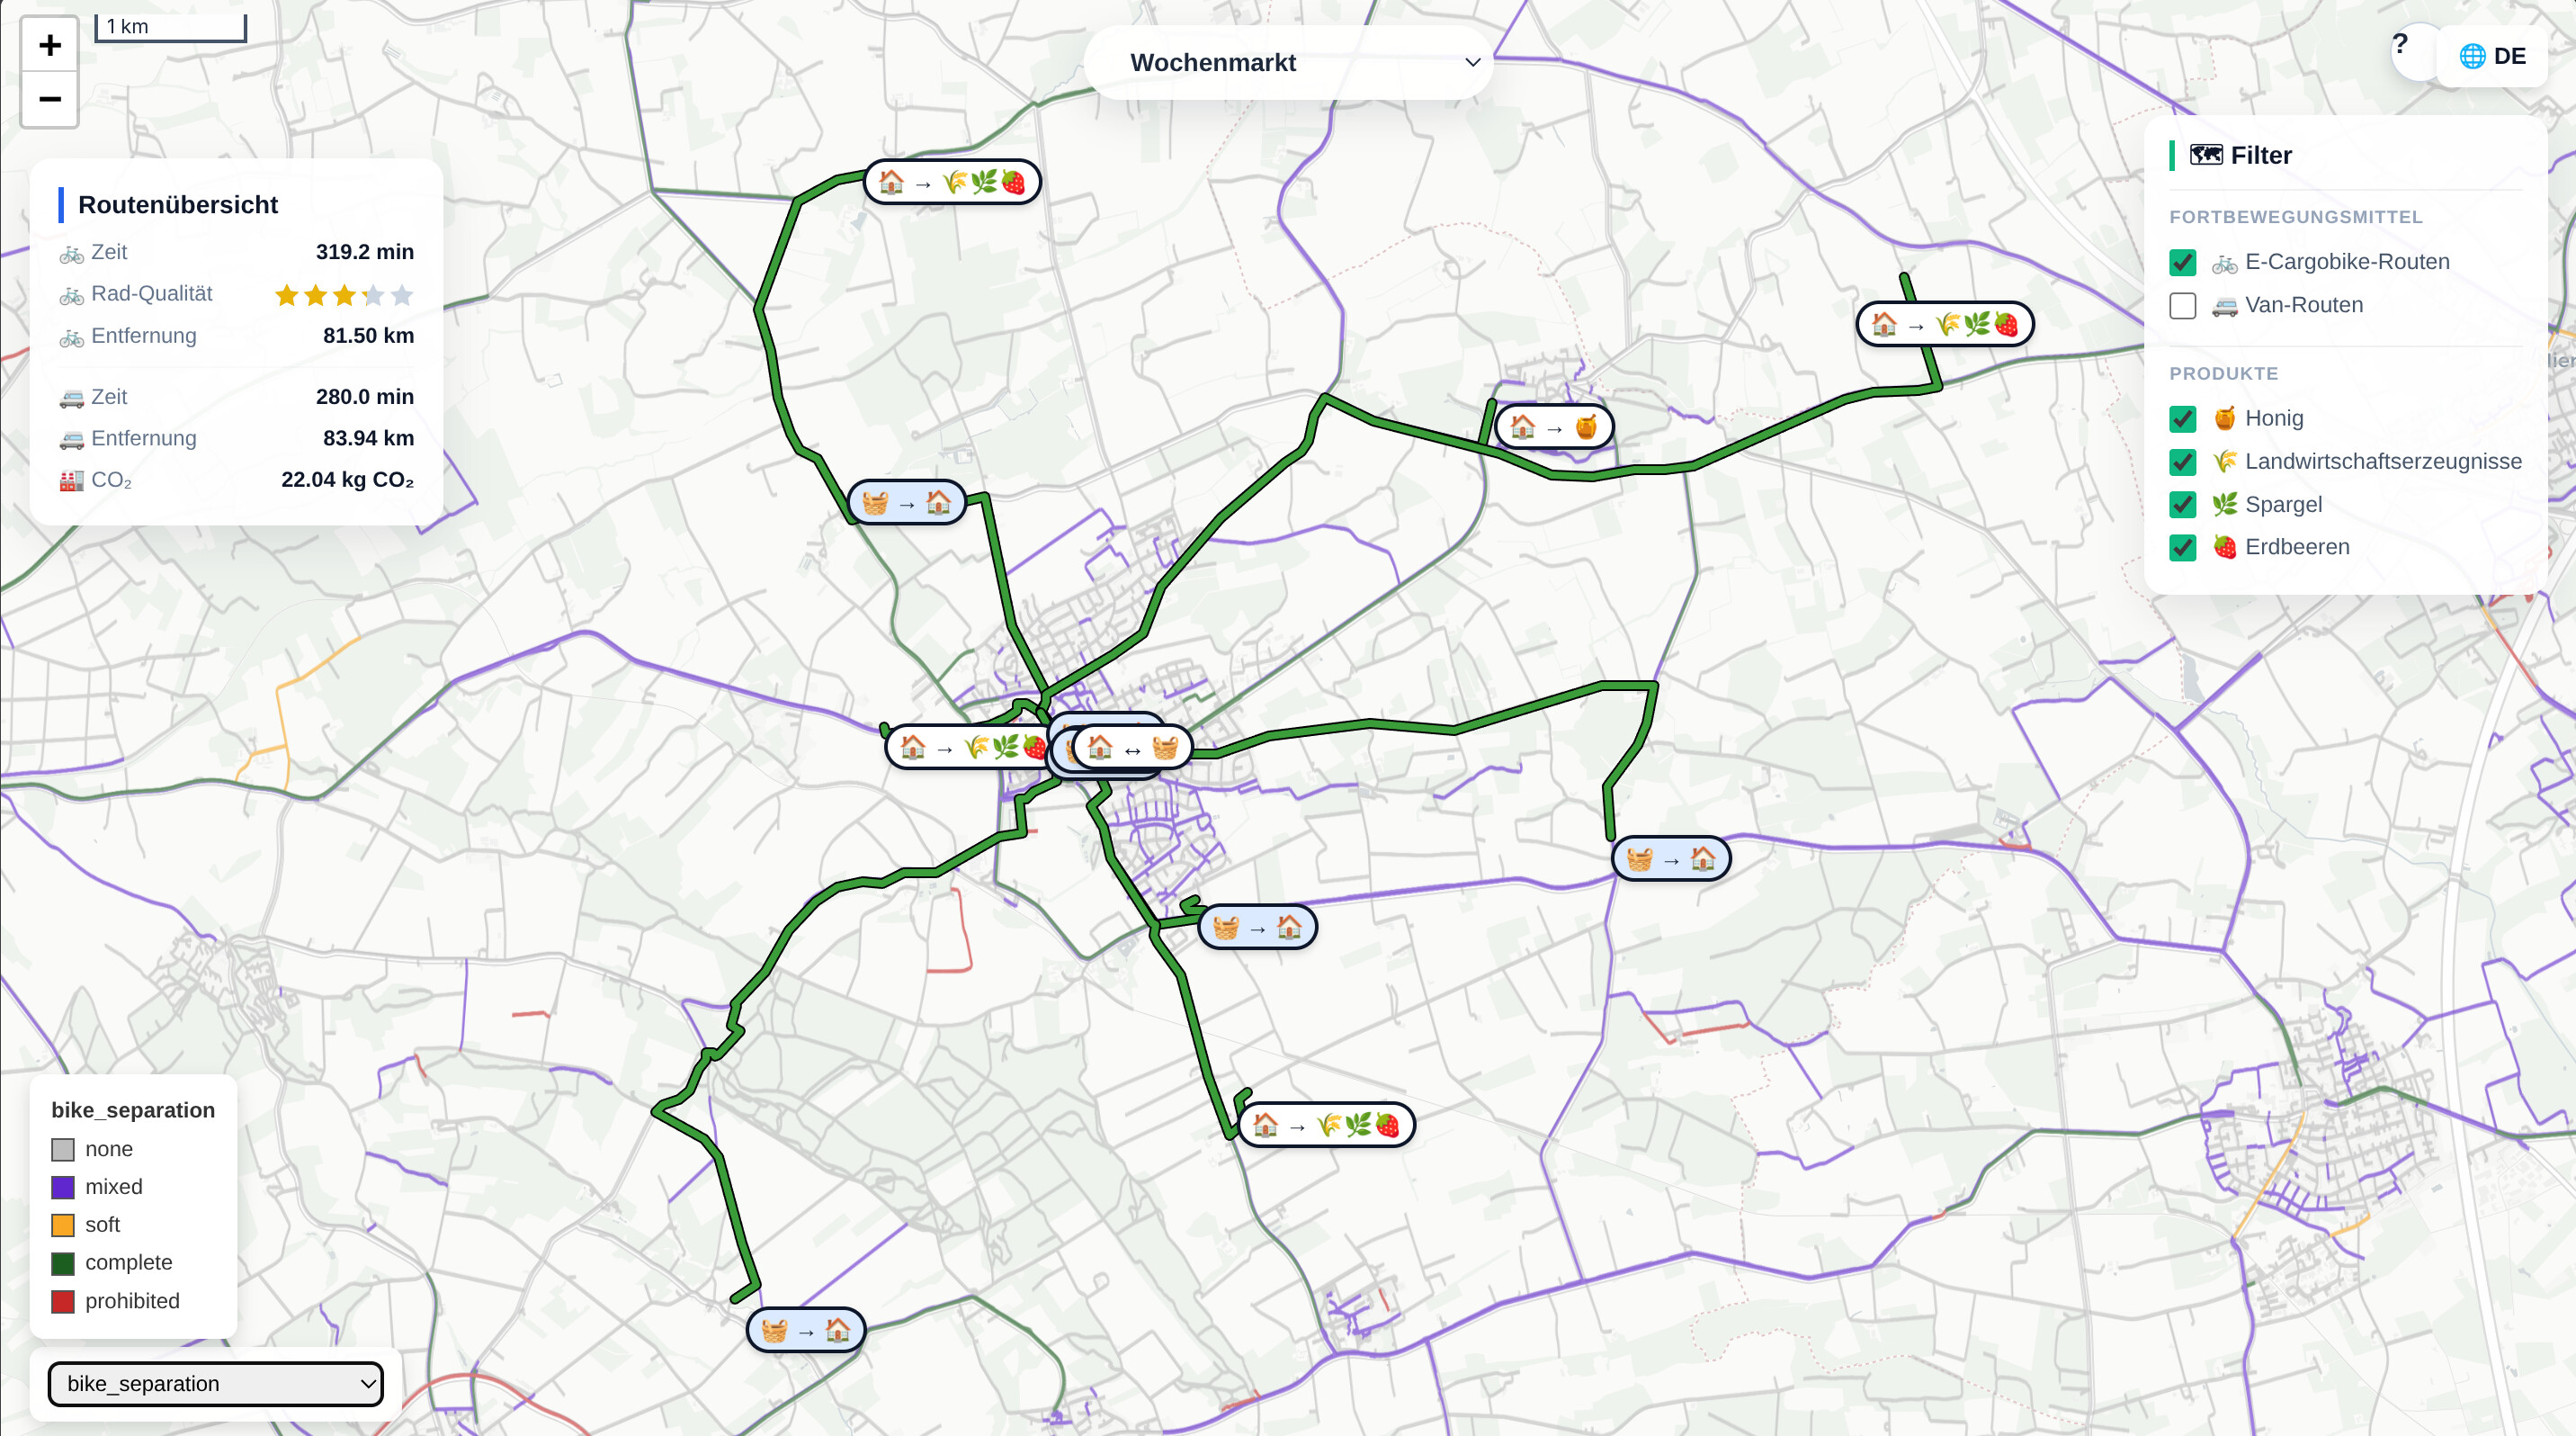
\includegraphics[width=0.75\textwidth]{figures/front_page.jpg}
\end{center}

\vspace{0.6cm}

\begin{flushleft}
\textbf{Verfasser}

Kana Mohammad

Urs Eble

Miguel Ureña Pliego
\end{flushleft}

\vfill

\begin{flushleft}
Frankfurt, 21.07.2026
\end{flushleft}

\vspace{0.5cm}
\begin{center}
Frankfurt University of Applied Sciences
\end{center}
\end{titlepage}

\pagenumbering{roman}

\chapter*{Zusammenfassung}
\addcontentsline{toc}{chapter}{Zusammenfassung}

Im ländlichen Raum wird ein Großteil kurzer Wege weiterhin mit dem Pkw zurückgelegt, obwohl sich viele davon grundsätzlich für Lastenräder eignen würden. Diese Arbeit untersucht am Beispiel der Gemeinde Havixbeck im Münsterland, wo genau dieses Potenzial für eine betriebliche Radlogistik liegt und wie groß es tatsächlich ist.

Zunächst wurde der Ist-Zustand der lokalen B2B-Logistik erfasst. Lokale Unternehmen wurden nach Branche, transportierten Gütern und Transportbeziehungen erhoben und anhand von Gewicht, Größe und besonderen Transportanforderungen bewertet. Auf dieser Grundlage wurden zwei Akteursgruppen mit besonders vielversprechenden Transportbeziehungen ausgewählt: das Stift Tilbeck als Produktions- und Logistikstandort sowie landwirtschaftliche Betriebe im Umland, die Wochenmärkte und Gastronomiebetriebe beliefern.

Da bestehende Routenplaner urbane Netze mit guter Tagging-Abdeckung voraussetzen und mit dem lückenhaft getaggten Straßennetz in Havixbeck schlecht umgehen, wurde eine eigene Routing-Engine entwickelt. Sie berechnet für Pkw und E-Lastenrad getrennt ein kinematisches Fahrzeitmodell, einen Bike-Score aus sechs Infrastrukturkriterien sowie eine kantenbasierte CO\textsubscript{2}-Bilanz und leitet daraus automatisch Liefertouren ab.

Auf dieser methodischen Grundlage wurden drei Konzepte entwickelt und ausgewertet: ein betriebseigenes Lastenrad für das Stift Tilbeck, ein betriebseigener Lastenanhänger für Direktlieferungen von Landwirtschaftsbetrieben an Gastronomien sowie ein Sharing-Lastenrad, mit dem Gastronomiebetriebe ihre Waren selbst abholen. Die Auswertung zeigt, dass Radlogistik vor allem bei kurzen, zentrumsnahen Strecken zeitlich konkurrenzfähig ist und dort auch ökologisch klar im Vorteil liegt, während sie mit zunehmender Entfernung an Wettbewerbsfähigkeit verliert. Das Stift Tilbeck erreicht dabei mit dem besten Bike-Score aller Konzepte das größte kurzfristige Umsetzungspotenzial. Beim Sharing-Konzept lohnt sich der Aufbau nur für eine kleine Gruppe zentrumsnaher Restaurants.

Insgesamt kann Radlogistik den Pkw in Havixbeck nicht flächendeckend ersetzen, ist aber an mehreren klar identifizierten Stellen bereits heute wirtschaftlich und ökologisch sinnvoll einsetzbar. Die Arbeit schließt mit konkreten Umsetzungsempfehlungen, etwa einem Pilotprojekt am Stift Tilbeck und Wochenmarkt sowie Anreizen für ein Sharing-System an den zentrumsnahen Standorten.

\tableofcontents

\listoffigures
\addcontentsline{toc}{chapter}{Bildverzeichnis}

\listoftables
\addcontentsline{toc}{chapter}{Tabellenverzeichnis}

\chapter*{Abkürzungsverzeichnis}
\addcontentsline{toc}{chapter}{Abkürzungsverzeichnis}
\begin{description}[labelwidth=2cm,leftmargin=2.8cm,style=nextline]
\item[B2B] Business-to-Business
\item[CO\textsubscript{2}] Kohlenstoffdioxid
\item[GPS] Global Positioning System
\item[HBEFA] Handbuch für Emissionsfaktoren des Straßenverkehrs
\item[HCM] Highway Capacity Manual
\item[LOS] Level of Service
\item[OSM] OpenStreetMap
\item[Pkw] Personenkraftwagen
\item[StVO] Straßenverkehrs-Ordnung
\item[TSP] Traveling Salesman Problem
\end{description}

\clearpage
\pagenumbering{arabic}

\chapter{Einleitung}

\section{Hintergrund und Anlass}

Der demografische Wandel in Deutschland führt zu einer zunehmenden Alterung der Bevölkerung. Bereits heute ist etwa jede zweite Person älter als 45 Jahre und rund jede fünfte älter als 66 Jahre. Der Anteil hochaltriger Menschen wird künftig weiter steigen \vgl{Destatis2025a}.

Besonders im ländlichen Raum ist dieser Effekt ausgeprägt: Dort ist der Anteil der über 65-Jährigen höher als in Städten (24\,\% gegenüber 19,6\,\%), was die Sicherstellung von Mobilität und Versorgung erschwert \vgl{Destatis2025b}.

Gleichzeitig ist die Mobilität in ländlichen Regionen stark durch den motorisierten Individualverkehr geprägt. So sind im ländlichen Raum Deutschlands 21\,\% aller Wege kürzer als 1\,km und weitere 11\,\% liegen zwischen 1 und 2\,km, dennoch werden selbst diese kurzen Distanzen häufig mit dem Pkw zurückgelegt. Bei Wegen unter einem Kilometer liegt der Anteil des motorisierten Verkehrs bereits bei rund 35\,\%, zwischen 1 und 2\,km sogar bei über 50\,\% \parencite{BMEL2023}. Dies führt zu erhöhten CO\textsubscript{2}-Emissionen, Lärm und Flächenverbrauch und steht im Widerspruch zu den Klimaschutzzielen Deutschlands \parencite{BMEL2023,KSG2019}.

Eine mögliche Lösung stellt der Einsatz von Lastenrädern dar. Insbesondere bei kurzen Distanzen und kleinteiligen Transporten können sie dazu beitragen, Verkehr zu verlagern, Emissionen zu reduzieren und die Mobilität nachhaltiger zu gestalten.

\section{Vorgehensweise und Methodik}

Die vorliegende Arbeit folgt einem systematischen Aufbau, der sich in drei zentrale Schritte gliedert. Zunächst erfolgt eine Analyse des Ist-Zustands der bestehenden Logistikstrukturen im Untersuchungsgebiet Havixbeck. Dabei werden relevante Akteure, Transportprozesse, Güterarten sowie eingesetzte Verkehrsmittel erfasst und bewertet.

Im Anschluss wird auf Basis dieser Analyse ein Radlogistikkonzept entwickelt. Hierbei werden geeignete Transportprozesse identifiziert, die auf Lastenräder verlagert werden können. Zudem erfolgt die Auswahl geeigneter Fahrzeugtypen sowie eine Betrachtung möglicher Routen und logistischer Strukturen, wie beispielsweise die Nutzung von Mikro-Hubs und die Bündelung von Gütern.

Die methodische Grundlage bildet eine Kombination aus Literaturrecherche, räumlicher Analyse sowie der Auswertung empirischer Daten aus dem Untersuchungsgebiet. Ergänzend werden logistische und technische Kriterien herangezogen, um die Eignung von Lastenrädern im Vergleich zum bestehenden System zu bewerten.

Abschließend wird der Ist-Zustand dem entwickelten Konzept gegenübergestellt, um Unterschiede, Potenziale sowie ökologische und betriebliche Effekte herauszuarbeiten.

\chapter{Ist-Zustand}

\section{Untersuchungsgebiet Havixbeck}

\begin{figure}[htbp]
\centering
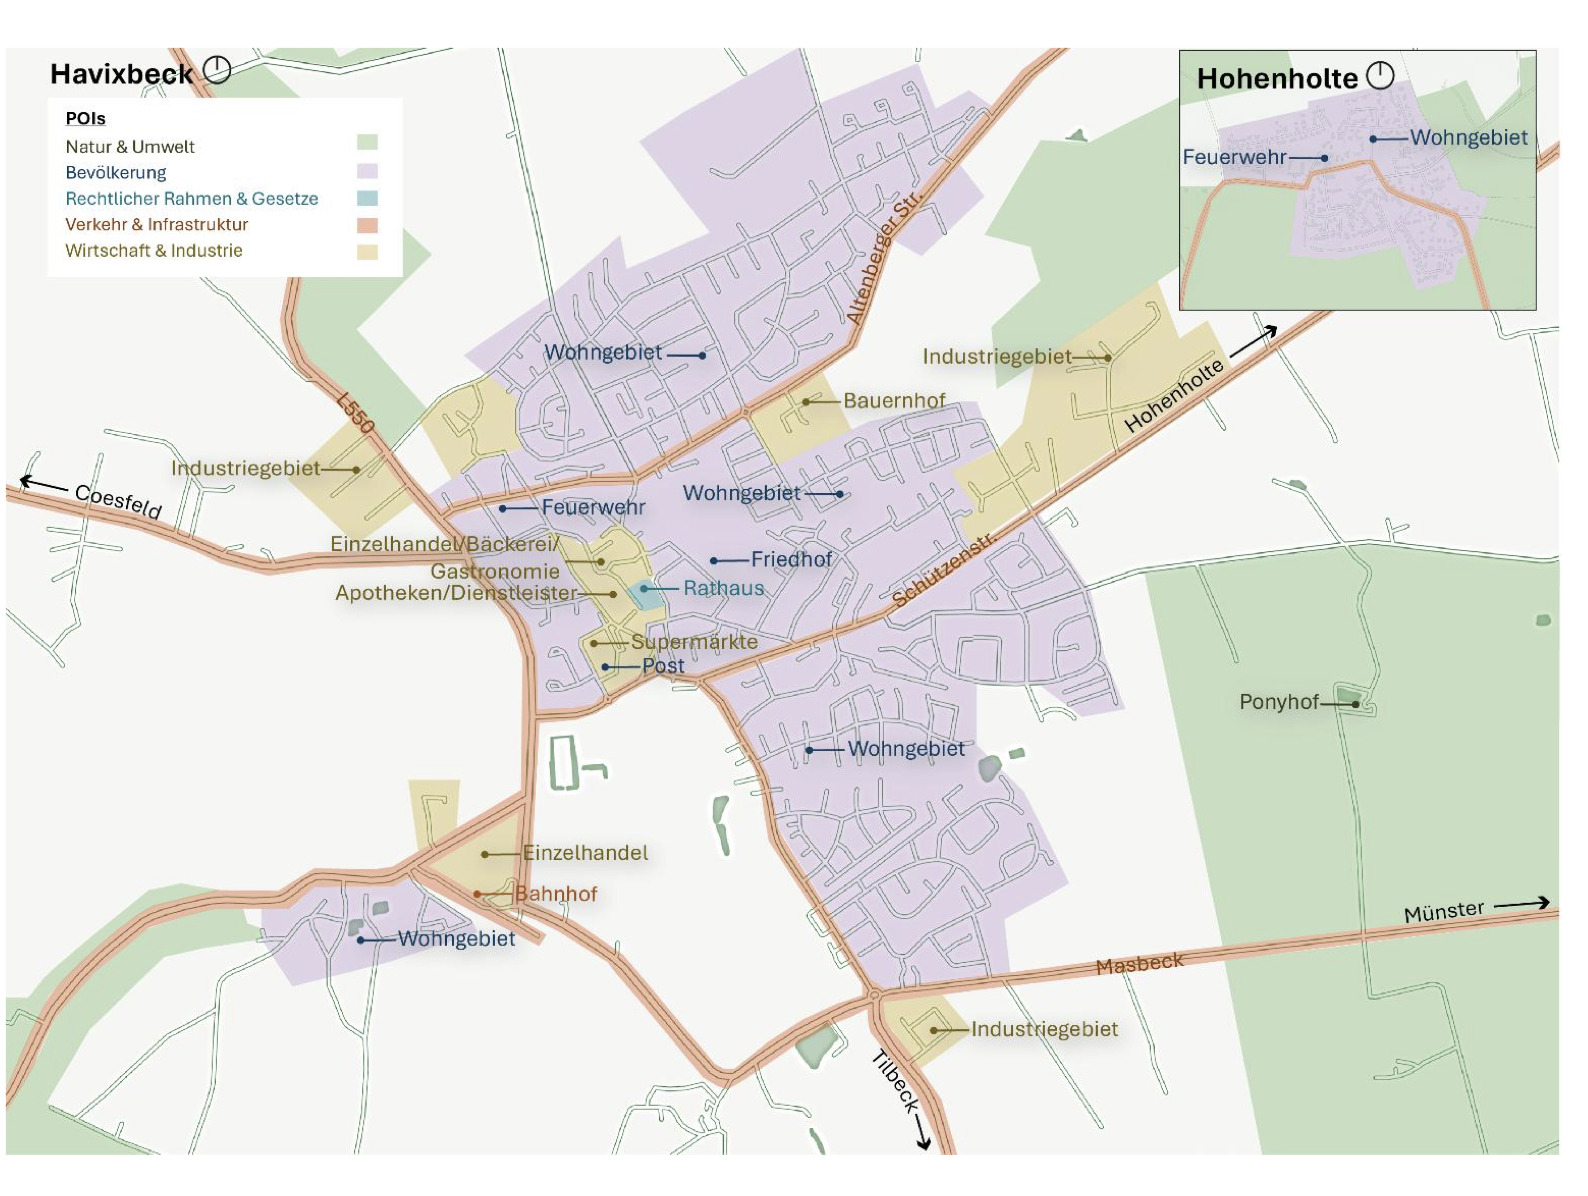
\includegraphics[width=0.85\textwidth]{figures/fig01_uebersichtskarte.jpg}
\caption[Übersichtskarte des Untersuchungsgebiets]{Übersichtskarte des Untersuchungsgebiets (Bildquelle: \cite{RADLAER2025})}
\label{fig:uebersichtskarte}
\end{figure}

Die Gemeinde Havixbeck liegt im westlichen Münsterland, etwa 15\,km von der Großstadt Münster entfernt, und zählt rund 12.000 Einwohner. Die Kommune ist ländlich geprägt, weist jedoch enge funktionale Verflechtungen mit Münster auf, insbesondere im Pendlerverkehr. Charakteristisch ist eine kompakte Siedlungsstruktur, bei der zentrale Alltagsziele wie Nahversorgung, Schulen und Verwaltung meist innerhalb von 2 bis 3\,km erreichbar sind. Dadurch bestehen grundsätzlich gute Voraussetzungen für den Einsatz des Fahrrads und insbesondere auch für Radlogistik. Gleichzeitig führen leichte topografische Unterschiede in den Baumbergen dazu, dass der Einsatz elektrisch unterstützter Fahrräder sinnvoll ist \vgl{RADLAER2025}. Bild~\ref{fig:uebersichtskarte} zeigt eine Übersichtskarte des Untersuchungsgebiets.

\section{Analyse der bestehenden Logistikstrukturen}

\begin{figure}[htbp]
\centering
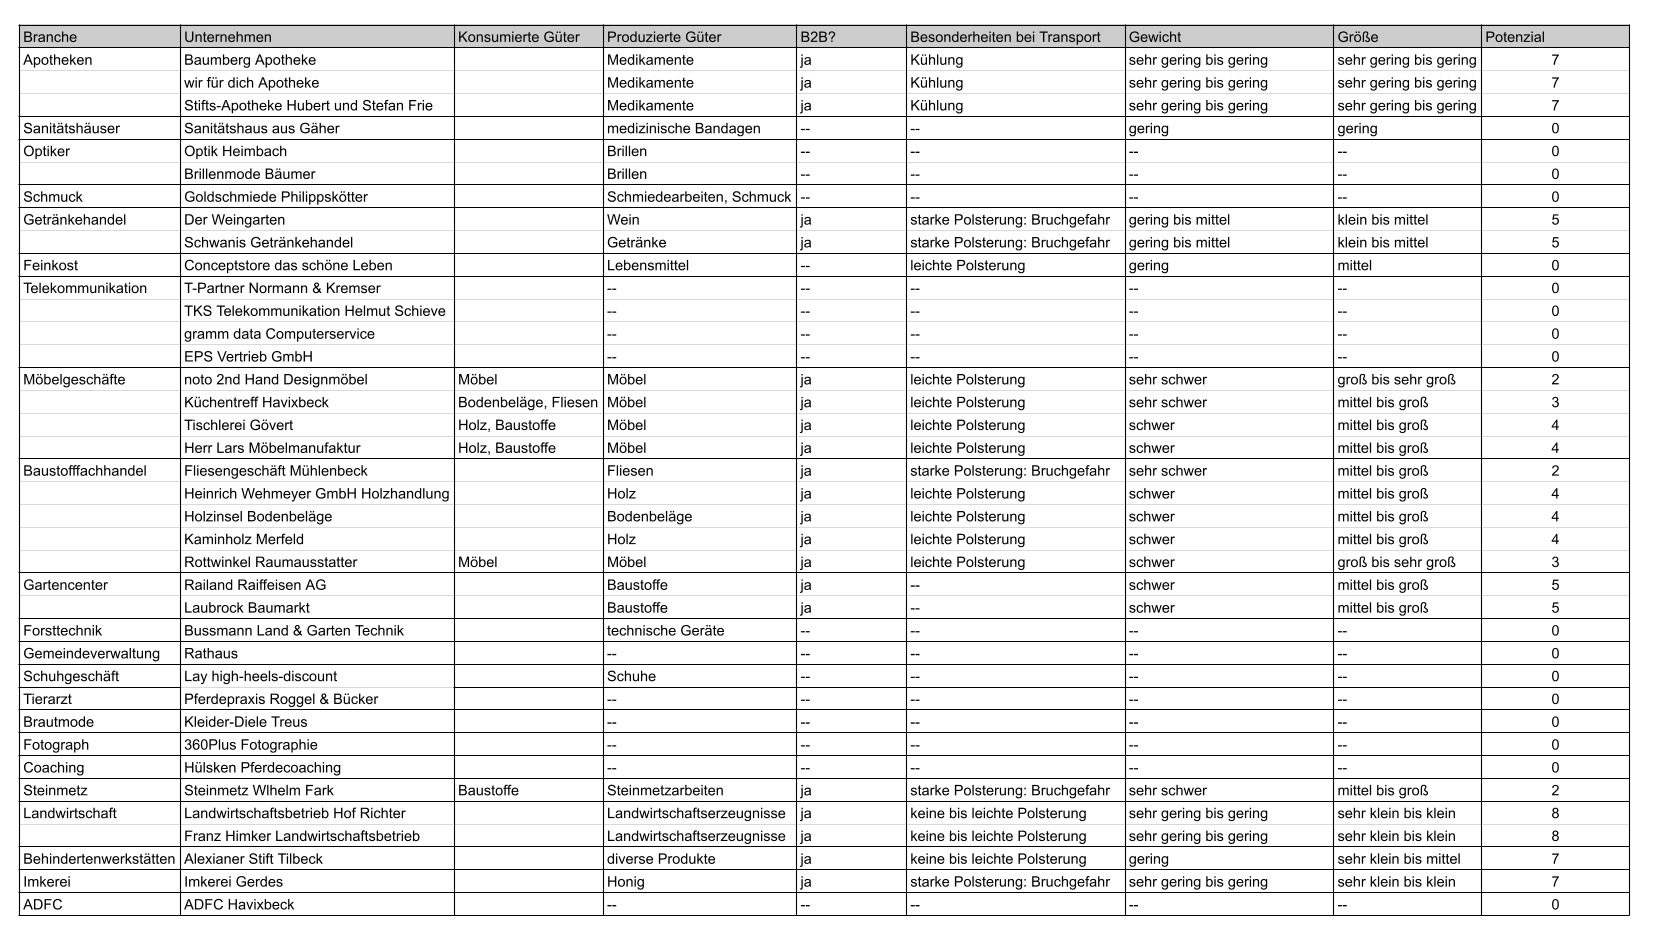
\includegraphics[width=\textwidth]{figures/fig02_bewertungstabelle.jpg}
\caption{Bewertungstabelle der einzelnen Unternehmen in Havixbeck}
\label{fig:bewertungstabelle}
\end{figure}

Auf Grundlage der räumlichen und strukturellen Gegebenheiten wurde der Ist-Zustand der Logistik im Untersuchungsgebiet erfasst. Hierfür erfolgte eine systematische Erhebung lokaler produzierender Akteure, die nach Branchen, Güterarten und Transportbeziehungen strukturiert wurde.

Die Analyse zeigt eine vielfältige Branchenstruktur mit unterschiedlichen logistischen Anforderungen. Während beispielsweise Apotheken leichte und teilweise kühlpflichtige Güter transportieren, dominieren im Baugewerbe schwere und großvolumige Waren wie Baustoffe oder Möbel.

Zur Bewertung der Eignung für Lastenräder wurde ein Punktesystem von 0 bis 10 verwendet. Die Bewertung erfolgte anhand der Kriterien Gewicht, Größe und Transportanforderungen sowie der Relevanz bestehender B2B-Transportbeziehungen. Unternehmen ohne B2B-Bezug wurden mit 0 Punkten bewertet.

Im Rahmen der Bewertung konnten die Unternehmen in den Kategorien Größe und Gewicht jeweils maximal fünf Punkte erreichen. Für beide Kategorien erfolgte die Punktevergabe auf einer fünfstufigen Skala, wobei kleinere beziehungsweise leichtere Ausprägungen höher bewertet wurden (sehr gering = 5 Punkte, gering = 4 Punkte, mittel = 3 Punkte, groß/schwer = 2 Punkte, sehr groß/sehr schwer = 1 Punkt). Da beide Kriterien gleich gewichtet wurden, ergab sich die Gesamtpunktzahl aus der Summe der in den beiden Kategorien erzielten Punkte.

Sofern für den Transport besondere Anforderungen bestanden, wurde ein Punktabzug vorgenommen. Erforderte der Transport eine Kühlung oder eine starke Polsterung, wurden zwei Punkte von der Gesamtpunktzahl abgezogen. War eine leichte Polsterung notwendig, wurde ein Punkt abgezogen.

Die Ergebnisse zeigen deutliche Unterschiede zwischen den Branchen. Leichte und kompakte Güter wie Medikamente oder bestimmte landwirtschaftliche Produkte eignen sich aufgrund kurzer Distanzen und einfacher Transportbedingungen gut für Lastenräder. Güter aus dem Bau- oder Möbelbereich weisen dagegen aufgrund ihres Gewichts und Volumens eine geringe Eignung auf.

Insgesamt zeigt die Ist-Analyse ein vorhandenes Potenzial für Radlogistik im Untersuchungsgebiet. Besonders bei kurzen Distanzen und leichten Gütern können Lastenräder eine nachhaltige Alternative zu bestehenden Transportlösungen darstellen. Bild~\ref{fig:bewertungstabelle} listet die Bewertung der einzelnen Unternehmen im Detail.

\chapter{Auswahl der Akteure}
\label{ch:auswahl}

Auf Grundlage der durchgeführten Ist-Analyse wurden zwei zentrale Akteure für eine vertiefende Untersuchung ausgewählt: das Stift Tilbeck sowie lokale landwirtschaftliche Betriebe.

\section{Stift Tilbeck}

\begin{figure}[htbp]
\centering
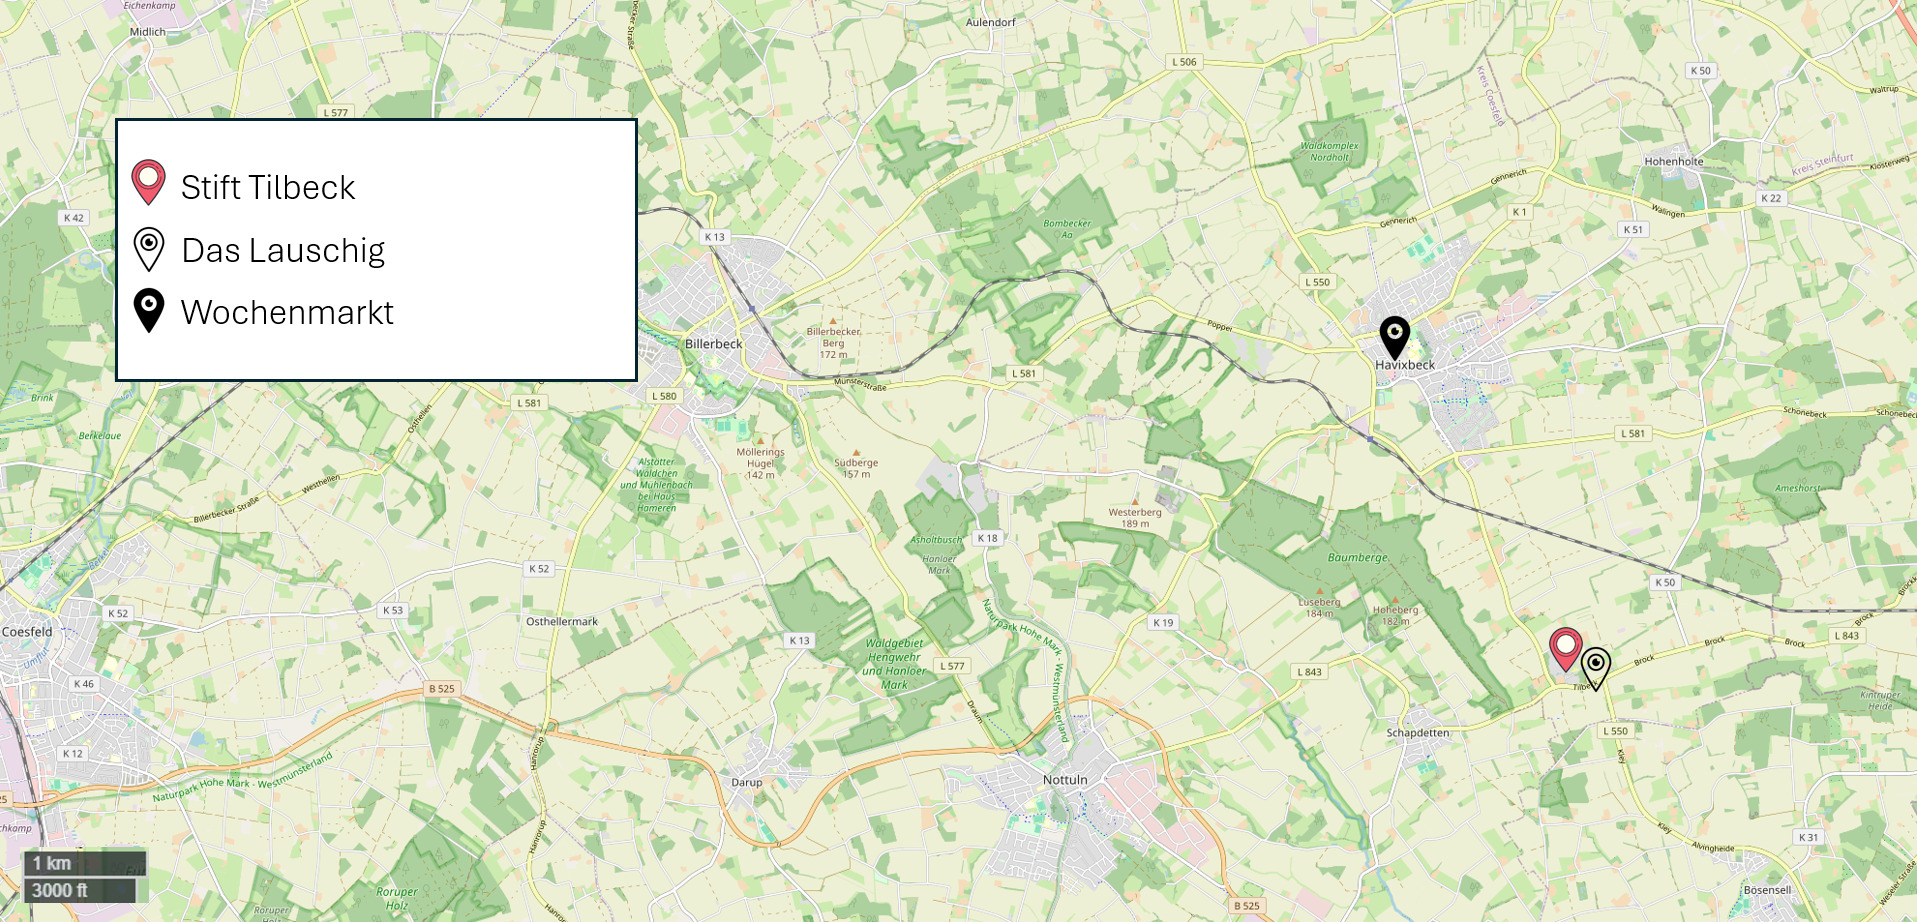
\includegraphics[width=0.85\textwidth]{figures/fig03_stift_tilbeck_bezugspunkte.jpg}
\caption[Relevante Bezugspunkte für Stift Tilbeck]{Darstellung der relevanten Bezugspunkte für Stift Tilbeck (Bildquelle: \cite{OpenStreetMap})}
\label{fig:stift-bezugspunkte}
\end{figure}


Das Stift Tilbeck ist ein bedeutender Produktions- und Logistikstandort im Untersuchungsgebiet. In verschiedenen Werkstätten stellen 80 Mitarbeiter und 371 betreute Personen Produkte aus Bereichen wie Textilien, Metallverarbeitung, Industriemontage, Kunsttherapie, Lettershop und Gärtnerei her \parencite{StiftTilbeck2026}. Zusätzlich übernimmt das Stift logistische Aufgaben, beispielsweise den Versand externer Aufträge.

Die Untersuchungen zeigten, dass nur ein Teil der Transporte für eine Radlogistik geeignet ist. Lieferungen und Abholungen für die Metall- und Industriemontage scheiden aufgrund von Gewicht, Volumen und Entfernung aus. Auch Produkte aus Textilproduktion, Lettershop und Kunsttherapie bieten aufgrund ihres Online-Vertriebs keinen geeigneten Ansatzpunkt.

Potenzial besteht hingegen bei den Transporten der Gärtnerei. Das Gemüse wird auf dem Gelände des Stifts, auf dem Havixbecker Wochenmarkt sowie im Restaurant „Das Lauschig“ verkauft. Die regelmäßigen Fahrten mit kurzen Distanzen und geeigneten Gütereigenschaften bieten gute Voraussetzungen für den Einsatz einer Radlogistik. Aktuell erfolgt der Transport zum Wochenmarkt mit einem Pkw und Anhänger. Bild~\ref{fig:stift-bezugspunkte} zeigt die relevanten Bezugspunkte.

\section{Landwirtschaftliche Betriebe}

\begin{figure}[htbp]
\centering
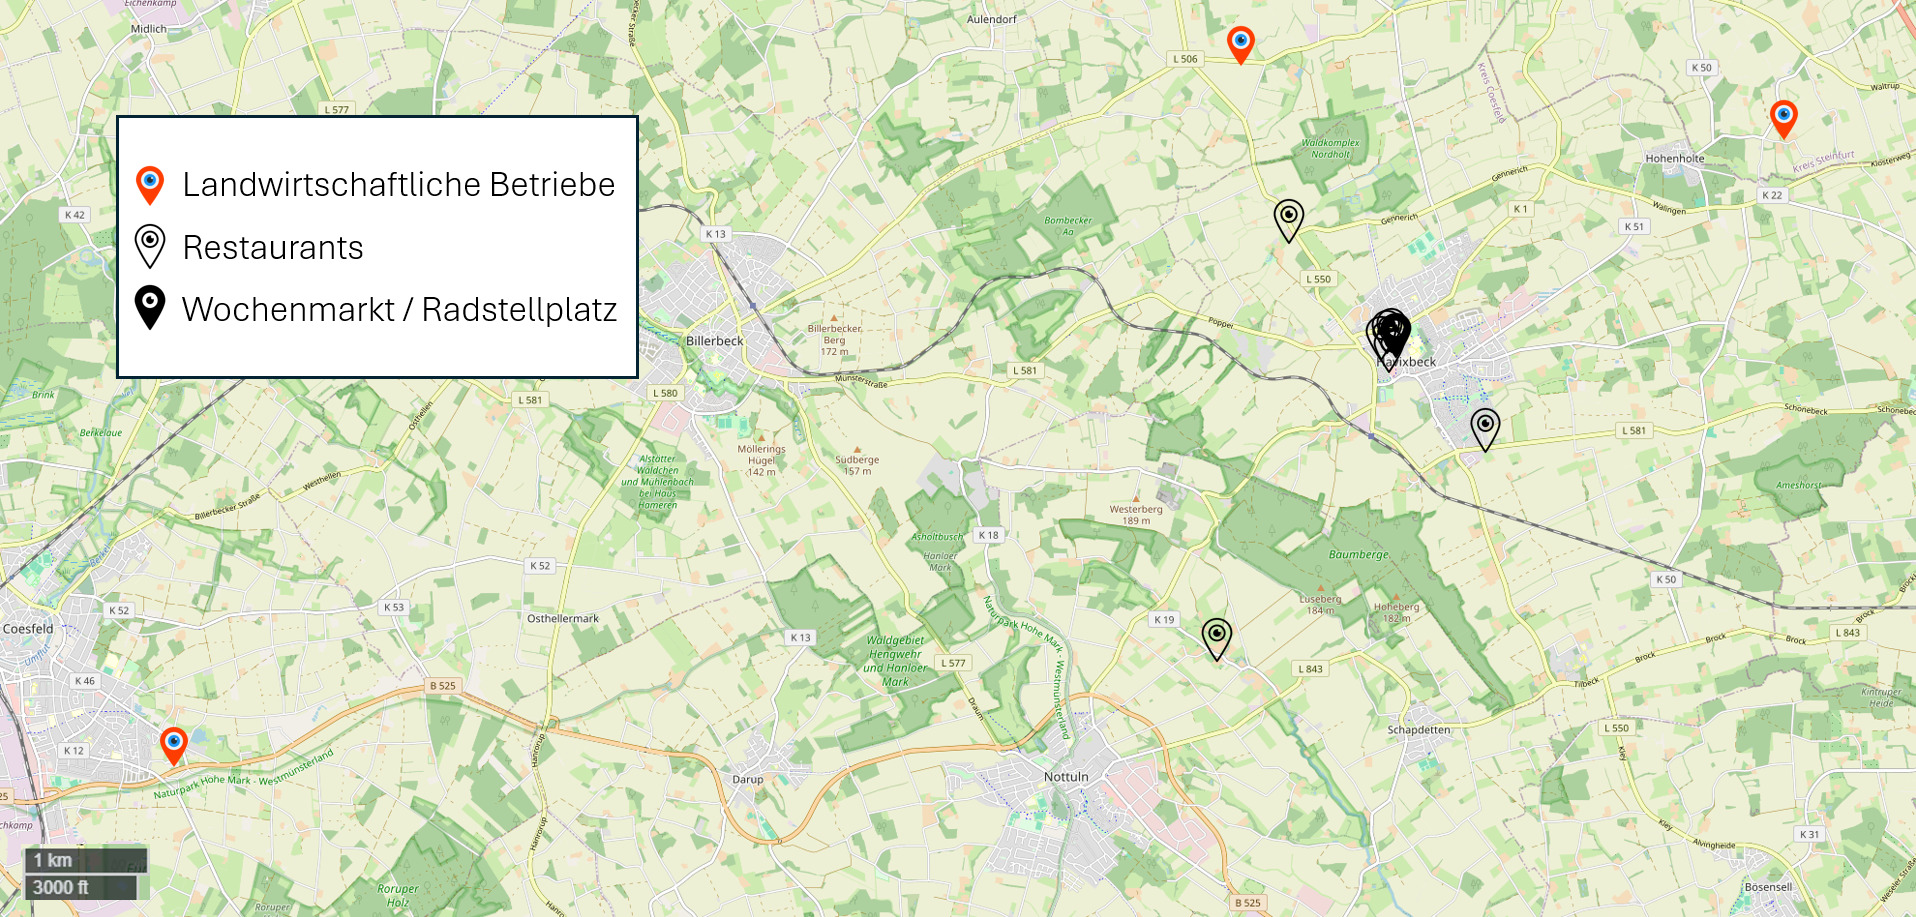
\includegraphics[width=0.85\textwidth]{figures/fig04_restaurants_landwirtschaft.jpg}
\caption[Restaurants und landwirtschaftliche Betriebe]{Darstellung der Restaurants und landwirtschaftlichen Betriebe (Bildquelle: \cite{OpenStreetMap})}
\label{fig:restaurants-landwirtschaft}
\end{figure}

Neben dem Stift Tilbeck wurden landwirtschaftliche Betriebe im Umland von Havixbeck als relevante Akteure identifiziert. Diese beliefern Wochenmärkte und lokale Gastronomiebetriebe mit regionalen Produkten. Aufgrund regelmäßiger Transporte und geeigneter Gütereigenschaften besteht grundsätzlich Potenzial für den Einsatz einer Radlogistik. Einschränkungen ergeben sich jedoch durch unterschiedliche Entfernungen zwischen Betrieben und Abnehmern sowie das unklare Interesse der Gastronomie.

Zur Ermittlung des Potenzials wurde eine telefonische Umfrage unter den Restaurants im Stadtgebiet durchgeführt, da keine verlässlichen Kontaktdaten der landwirtschaftlichen Betriebe vorlagen. Von den acht Restaurants konnten fünf erreicht werden. Die Befragung umfasste folgende Fragen:

\begin{enumerate}
\item Von welchen Quellen erhalten Sie aktuell Ihre Produkte?
\item Falls Sie Produkte von landwirtschaftlichen Betrieben aus der Nähe erhalten, um welche Produkte handelt es sich?
\item Falls Sie Produkte von landwirtschaftlichen Betrieben aus der Nähe erhalten, von welchen Betrieben kommen die Produkte?
\item Wie häufig findet die Belieferung durch landwirtschaftliche Betriebe statt?
\end{enumerate}

Vier der fünf befragten Restaurants beziehen neben dem Großhandel auch regionale Produkte, während ein Restaurant ausschließlich über den Großhandel versorgt wird. Die regional bezogenen Produkte beschränken sich überwiegend auf saisonale Erzeugnisse wie Spargel oder Erdbeeren. Als konkrete Lieferbetriebe wurden Hof Baumeister in Altenberge, Hof Heilers-Lülf in Billerbeck und Hof Rahmann in Coesfeld-Harle genannt. Aufgrund der saisonalen Abhängigkeit konnten keine verlässlichen Aussagen zur Lieferfrequenz getroffen werden. Bild~\ref{fig:restaurants-landwirtschaft} zeigt die Lage der Restaurants und landwirtschaftlichen Betriebe.

\chapter{Routing}
\label{ch:routing}

\section{Warum eine eigene Routing-Engine entwickelt wurde}

Bestehende OSM-Router (OSRM, GraphHopper, BRouter, CycleStreets) sind für urbane Netze mit guter Tagging-Abdeckung optimiert \parencite{Luxen2011,GraphHopper,Brenschede,CycleStreets}. In Havixbeck sind viele Attribute nicht getaggt, sodass Black-Box-Router damit schlecht umgehen. Deshalb wurde mit OSMnx/NetworkX eine eigene Routing-Pipeline gebaut: volle Kontrolle über Straßennetz, Bewertungskriterien und Parameter, plus ein eigener Bikeability-Score pro Kante. Defaults für fehlende Tags wurden auf das Gebiet abgestimmt, statt urban kalibrierte Logik zu übernehmen. Die berechneten Routen wurden stichprobenartig mit Google Maps verglichen.

\section{Aufbau der Routing-Engine}

Für jede Kante werden getrennt für Pkw und (E-)Lastenrad eine Fahrzeit und ein Score berechnet. Die beste Route folgt daraus mit dem Dijkstra-Algorithmus.

\subsection{Kinematisches Fahrzeitmodell}

Statt Distanz und Höchstgeschwindigkeit nutzt die Engine ein Geschwindigkeitsprofil mit Beschleunigung, Cruising und Verzögerung \parencite{May1990,TRB2022}. Jeder Kreuzung wird ein Node Penalty zugeordnet, wie in der Literatur zu Abbiegewiderständen an Kreuzungen üblich \parencite{Kirby1969,Winter2002,Ziliaskopoulos1996}: 2\,s (Pkw) bzw. 0,5\,s (E-Bike) unsignalisiert \parencite{Mohammadi2023}, 15\,s signalisiert nach dem Highway Capacity Manual \parencite{TRB2022}. Die gewählten Werte liegen jeweils im mittleren Bereich der in der Literatur berichteten Spannen. Havixbeck hat laut OpenStreetMap nur zwei signalisierte Kreuzungen \parencite{OpenStreetMap}.

Die Beschleunigung ist beim E-Bike höher als beim Pkw angesetzt (1,5--2,5\,m/s\textsuperscript{2}), weil der Elektromotor sofort das volle Drehmoment liefert und das Lastenrad ein deutlich geringeres Gewicht als ein Pkw beschleunigen muss. Höchstgeschwindigkeiten folgen meistens der Straßenverkehrs-Ordnung: 7\,km/h Schrittgeschwindigkeit im verkehrsberuhigten Bereich, sonst 25\,km/h für das E-Lastenrad \parencite{StVO2013}. Auf mit Fußgängern geteilten Wegen setzt die Engine 10\,km/h an, da dort mehr Konflikte auftreten und höhere Geschwindigkeiten unsicher wären. Der Pkw nutzt die aus dem OSM-Typ abgeleitete Höchstgeschwindigkeit (20--100\,km/h).

Das kinematische Fahrzeitmodell berücksichtigt keine Steigung, was vertretbar ist, weil das E-Lastenrad ohnehin von einem Elektromotor unterstützt wird, der Höhenunterschiede beim Beschleunigungs- und Cruisingverhalten weitgehend ausgleicht, und weil Havixbeck und sein Umland ein sehr flaches Relief mit nur geringen Höhenunterschieden aufweisen.

\subsection{Straßentyp-Präferenz beim Pkw-Routing}

Das Pkw-Routing bevorzugt zusätzlich höherrangige Straßen (Autobahnen/Landstraßen) -- ein Präferenzverhalten, das in der Verkehrszuordnung (Assignment) allgemein modelliert wird \parencite{Ortuzar2011} --, selbst wenn die Fahrzeit dadurch im Modell bis zu 10\,\% länger ausfällt. So laufen Pkw- und Radrouten oft auseinander: Der Pkw nimmt die Umgehung, das Lastenrad fährt direkt durch den Ortskern oder nutzt für den Pkw gesperrte Feldwege. Bild~\ref{fig:routenvergleich1} zeigt ein Beispiel dieser Abweichung.

\begin{figure}[htbp]
\centering
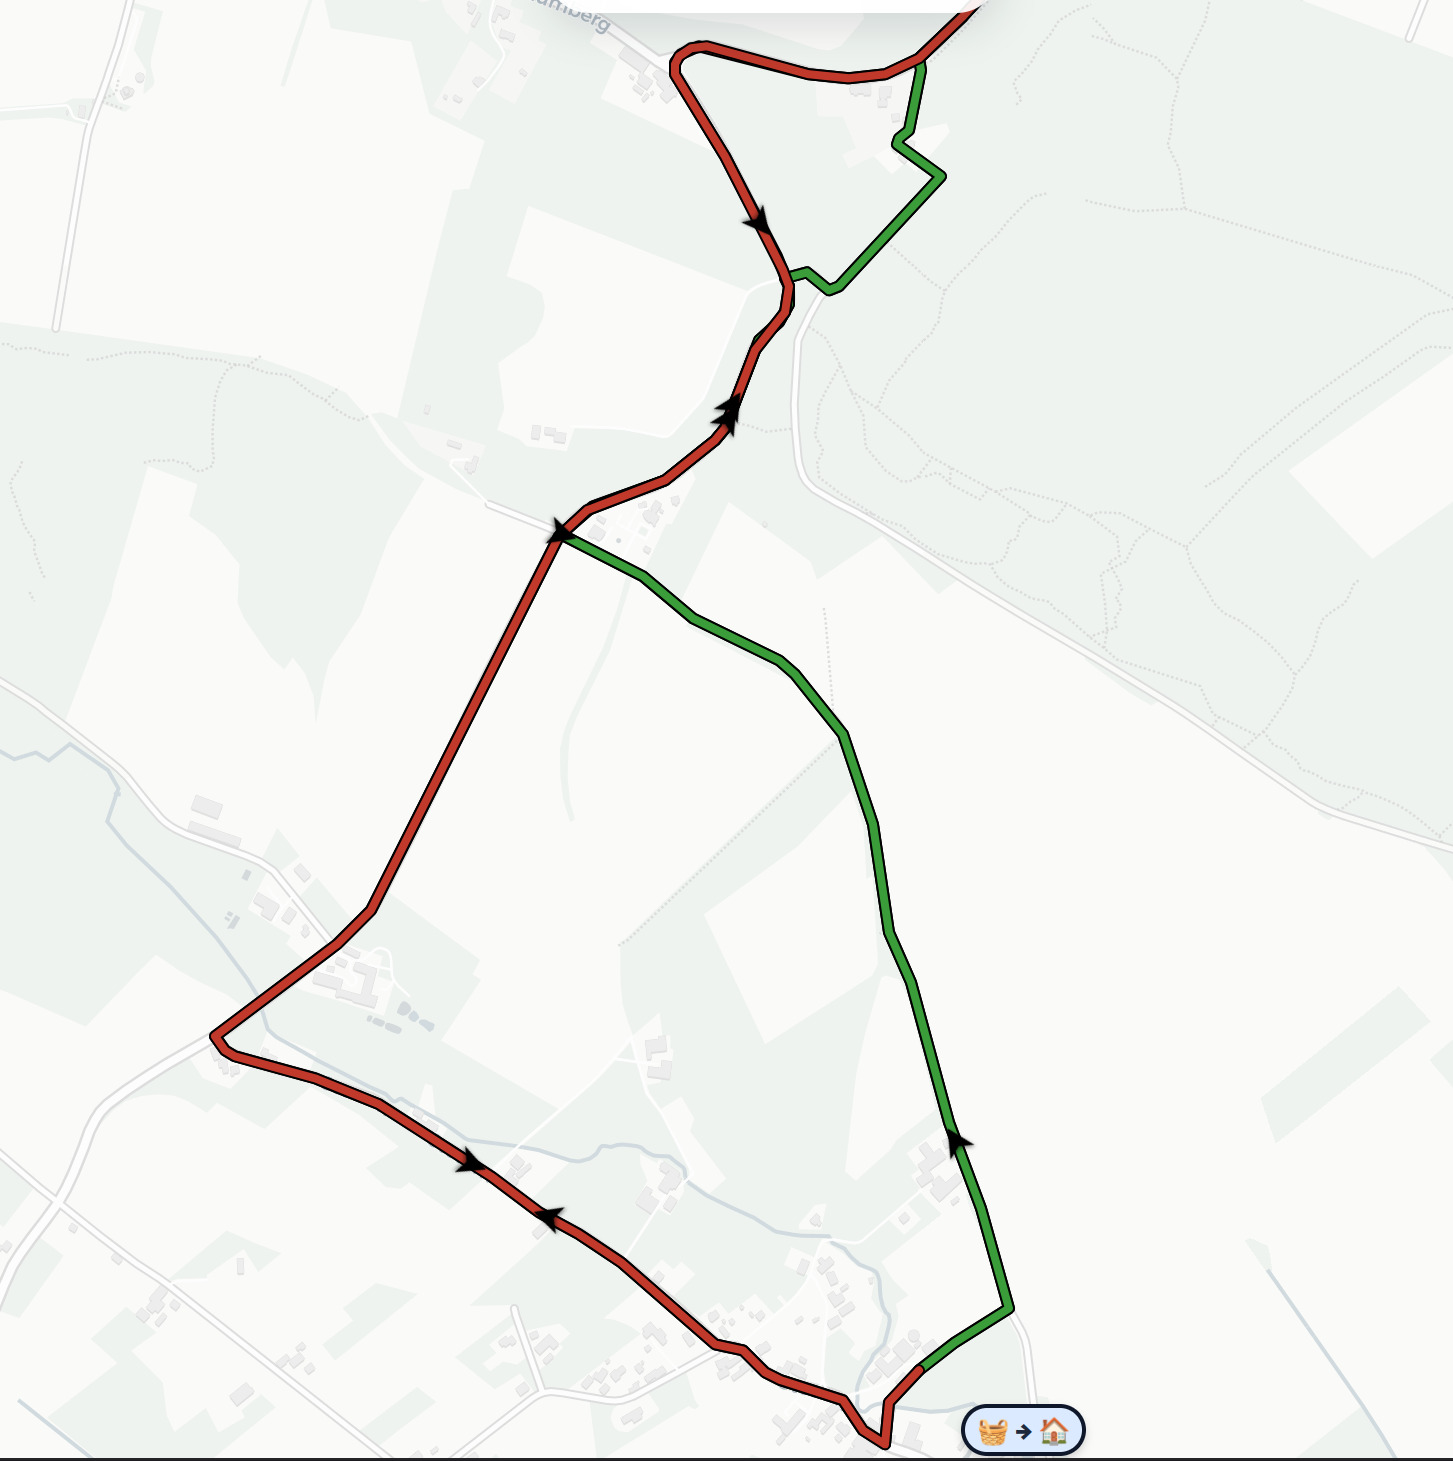
\includegraphics[width=0.55\textwidth]{figures/fig05_routenvergleich_auto_rad.jpg}
\caption[Routenvergleich Auto vs.\ Fahrrad]{Unterschiede in einer Route: Auto (rot) und Fahrrad (grün) (eigene Darstellung, Datenquelle: \cite{OpenStreetMap}\interaktivekarte)}
\label{fig:routenvergleich1}
\end{figure}

\subsection{Bike-Score und wahrgenommene Fahrzeit}

Der Bike-Score (0--10) wird aus sechs gewichteten Kriterien berechnet (Tabelle~\ref{tab:bikescore}).

{\small
\begin{longtable}{@{}p{3.1cm}p{1.3cm}p{6.5cm}p{1.4cm}@{}}
\caption{Bike-Score-Kriterien}\label{tab:bikescore}\\
\toprule
\textbf{Kriterium} & \textbf{Gewicht} & \textbf{Wertebereich} & \textbf{Default} \\
\midrule
\endfirsthead
\multicolumn{4}{@{}l}{\small\itshape Fortsetzung von der vorherigen Seite}\\
\toprule
\textbf{Kriterium} & \textbf{Gewicht} & \textbf{Wertebereich} & \textbf{Default} \\
\midrule
\endhead
\midrule
\multicolumn{4}{@{}r}{\small\itshape Fortsetzung auf der nächsten Seite}\\
\endfoot
\bottomrule
\endlastfoot
Trennung vom Kfz-Verkehr & 10 & baulich getrennt = 10, mitgeführt = 5, keine Trennung = 1 & 1 \\
Straßentyp & 10 & Wohn-/Feldweg/Radweg = 10, Erschließungsweg = 8, Weg = 7, Fuß-/Reitweg = 5, drittrangige Straße = 3, zweitrangige Straße = 2, Haupt-/Fernstraße = 1 & 5 \\
Zugangsbeschränkung & 10 & Fußgänger+Rad/Erlaubnis/Anwohner = 10, privat/nur Fußgänger = 1 & 5 \\
Kfz-Geschwindigkeit & 10 & 0--5\,km/h = 10, 20\,km/h = 8, 30\,km/h = 5, 50\,km/h = 1 & 5 \\
Fahrbahnoberfläche & 5 & Asphalt/Beton = 10, Kopfsteinpflaster = 5, unbefestigt = 1 & 10 \\
Fahrspuren & 5 & 1 Spur = 10, 2 Spuren = 5, 3+ Spuren = 1 & 10 \\
\end{longtable}
}

Die drei Gewicht-10-Kriterien dominieren, konsistent mit Trennung und Straßenklasse als stärksten Einflussfaktoren \parencite{Broach2012}. Defaults stammen aus Sichtprüfung von Stichproben. Ein Ignore-Mechanismus blendet nicht aussagekräftige Kriterien aus, angelehnt an das „Level of Traffic Stress“-Konzept \parencite{Furth2016} und CycleStreets' „Quietness“-Wert \parencite{CycleStreets}. Die Bilder~\ref{fig:pavement} und~\ref{fig:bikescore-werte} zeigen die daraus resultierenden Pavement- und Bike-Score-Werte im Untersuchungsgebiet.

\begin{figure}[htbp]
\centering
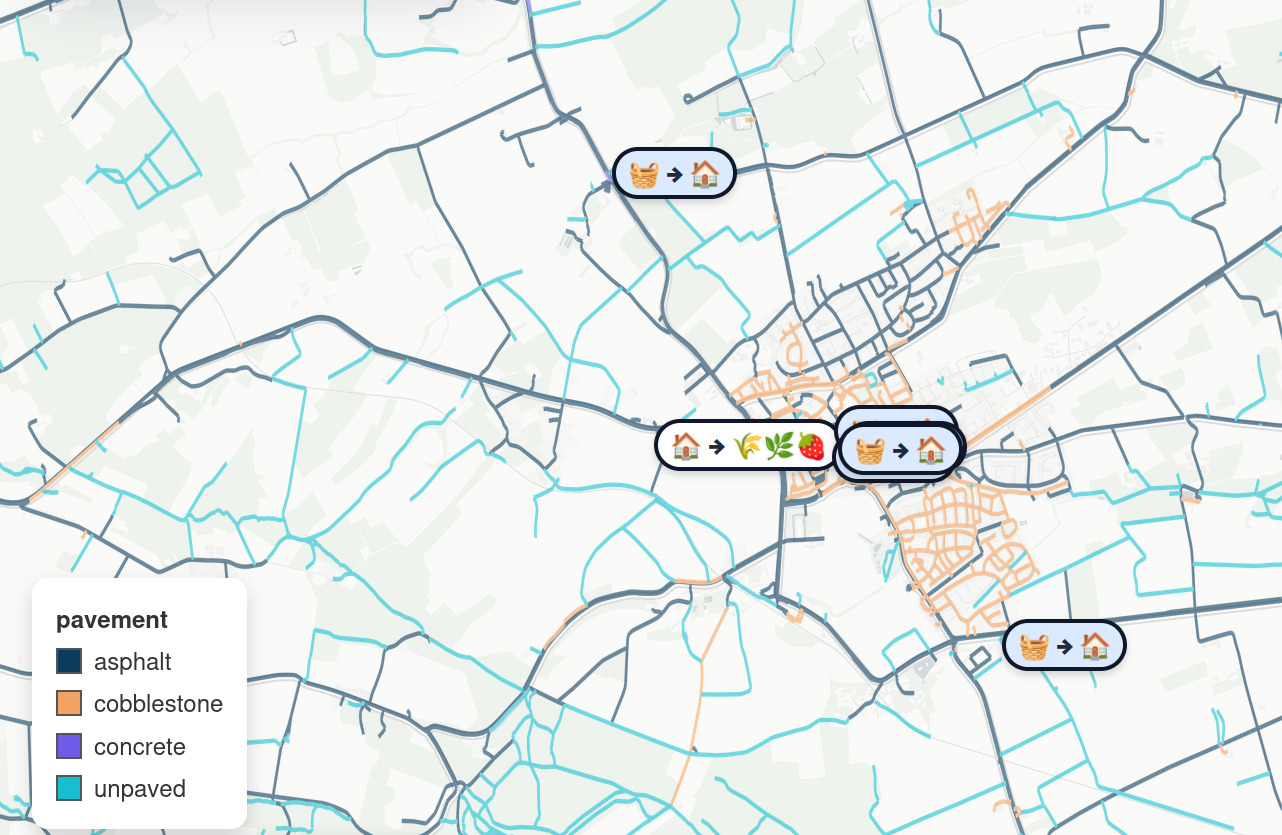
\includegraphics[width=0.65\textwidth]{figures/fig06_pavement_werte.jpg}
\caption[Pavement-Werte in Havixbeck]{Pavement-Werte in Havixbeck (eigene Darstellung, Datenquelle: \cite{OpenStreetMap}\interaktivekarte[Pavement][raster=pavement])}
\label{fig:pavement}
\end{figure}

\begin{figure}[htbp]
\centering
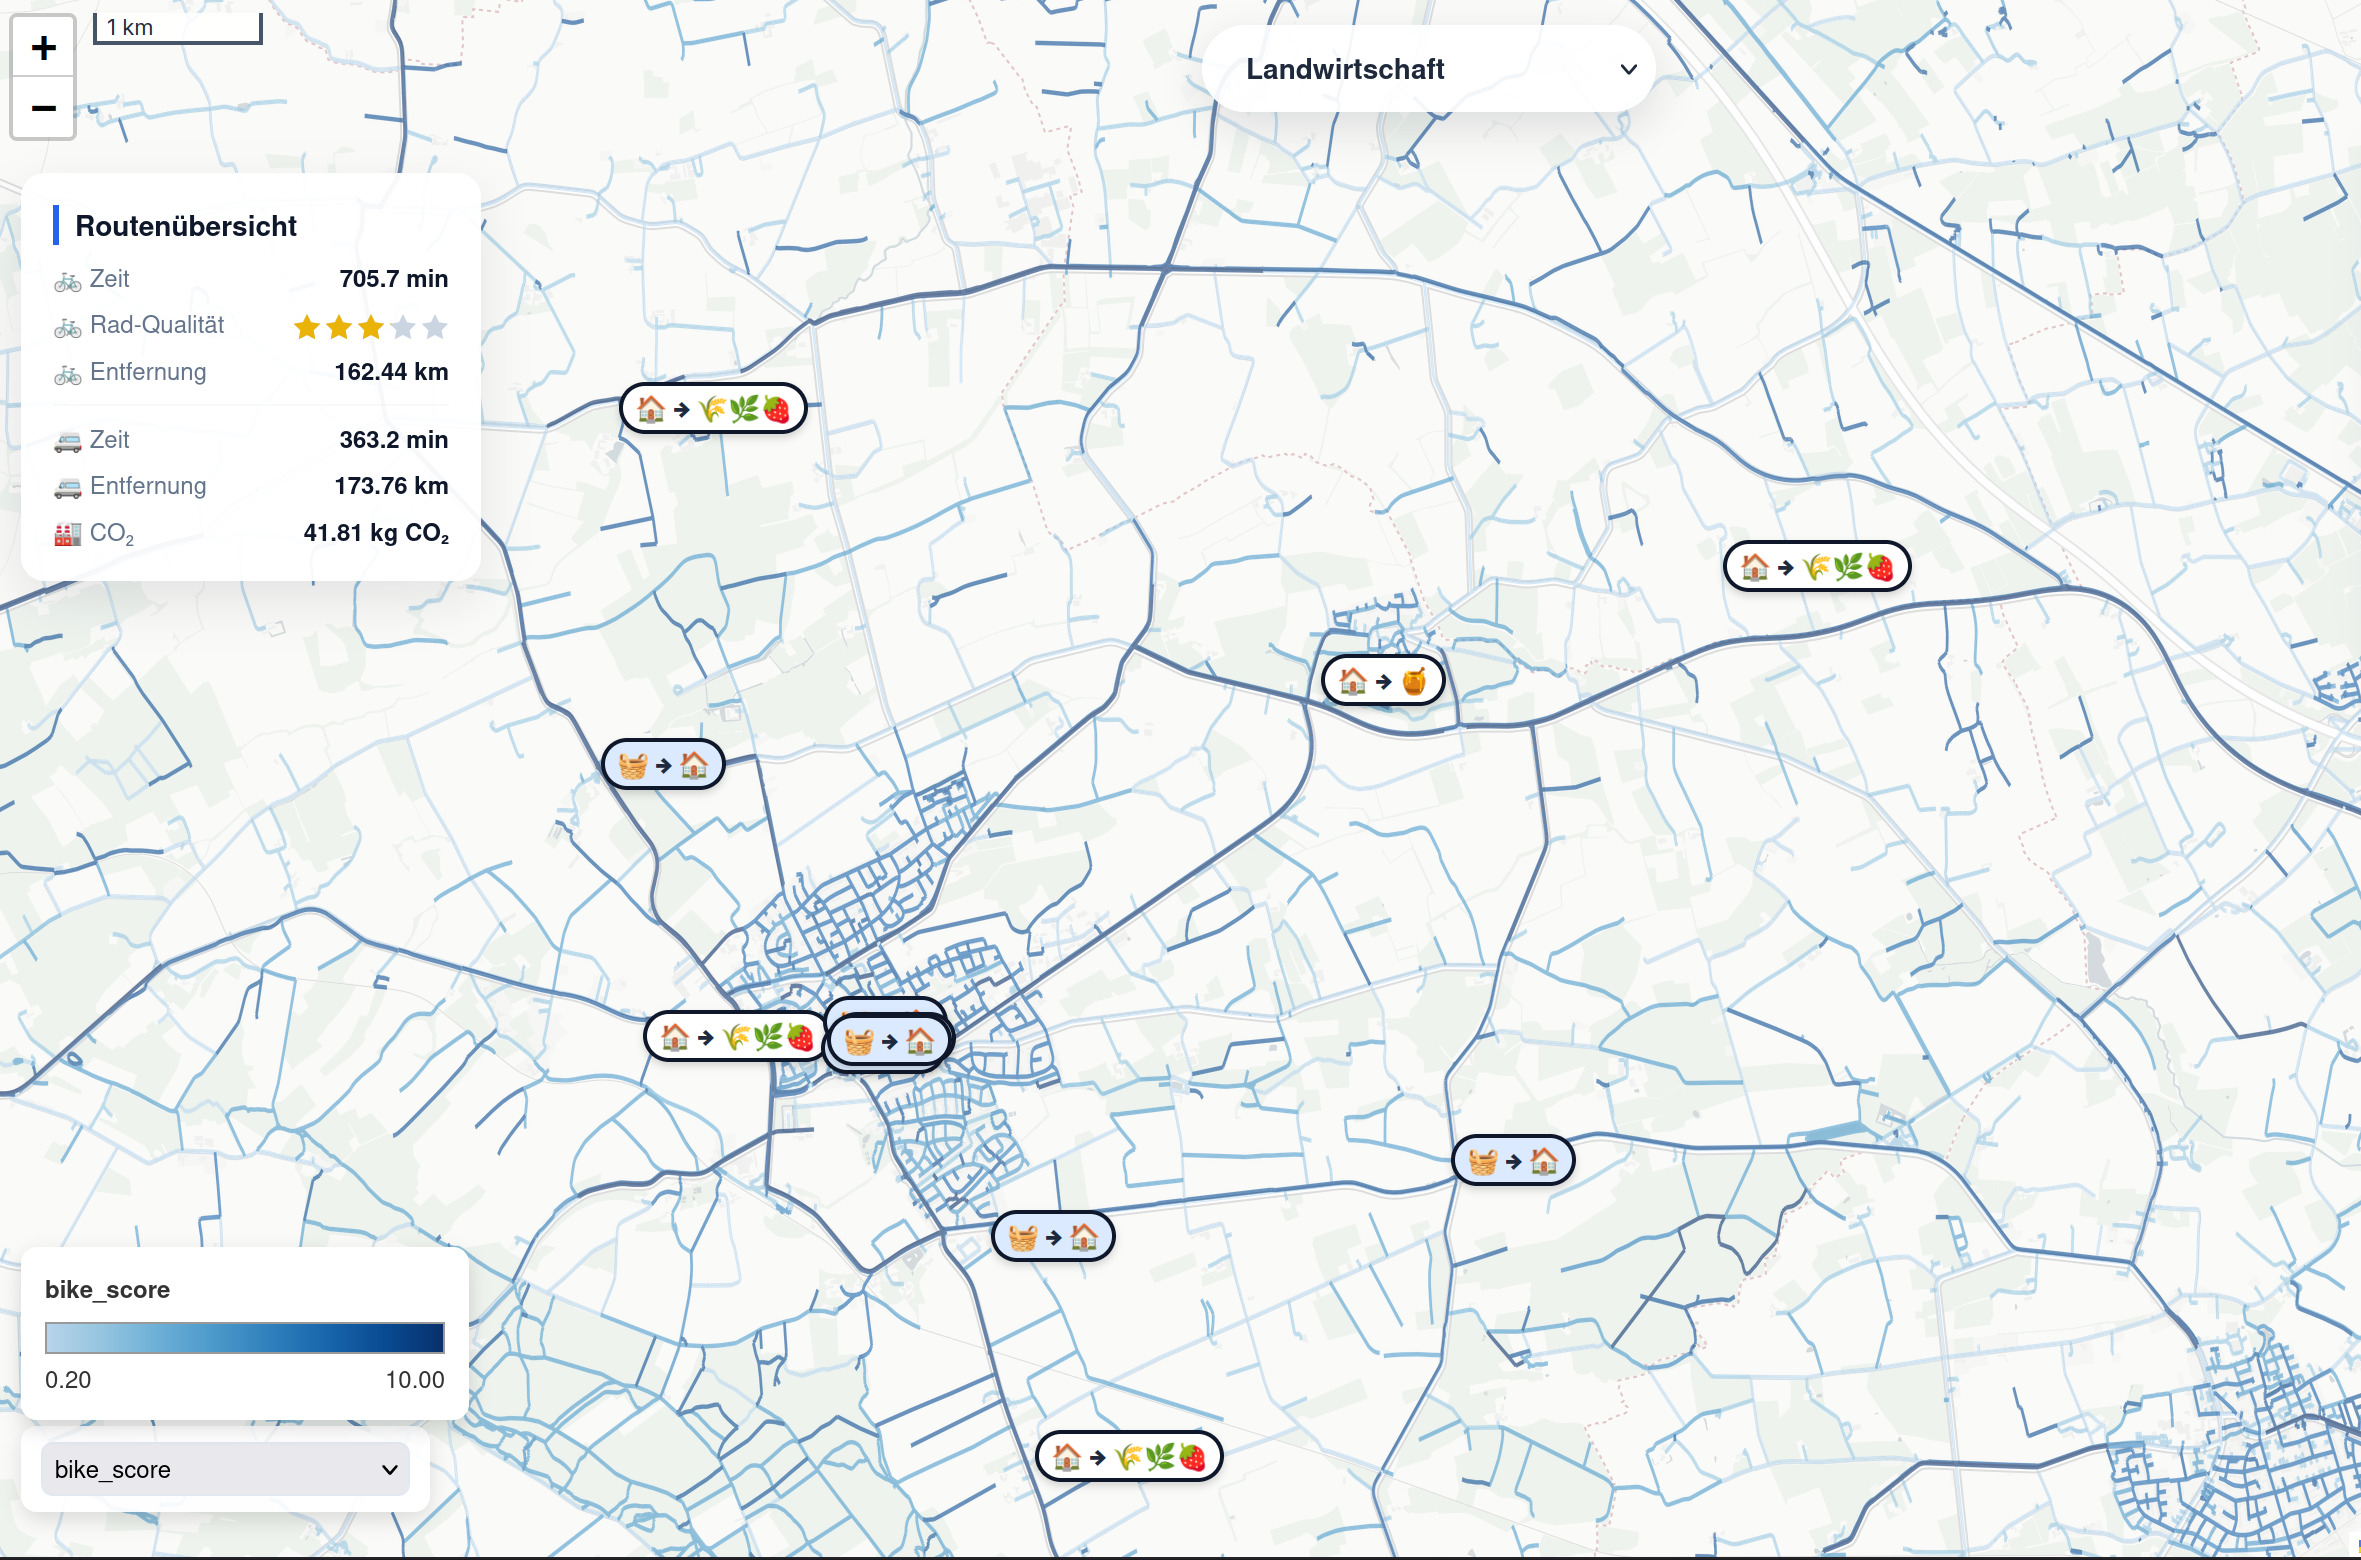
\includegraphics[width=0.65\textwidth]{figures/fig07_bikescore_werte.jpg}
\caption[Bike-Score-Werte in Havixbeck]{Bike-Score-Werte in Havixbeck (eigene Darstellung, Datenquelle: \cite{OpenStreetMap}\interaktivekarte[Bike-Score][raster=bike_score])}
\label{fig:bikescore-werte}
\end{figure}

Die wahrgenommene Fahrzeit $t_{\text{wahrg.}}$ ergibt sich aus der kinematischen Fahrzeit $t_{\text{kin.}}$, gewichtet mit dem Bike-Score $b$ und einem Reduktionsfaktor $r$:

\begin{equation}
t_{\text{wahrg.}} = t_{\text{kin.}} \cdot \left( w - \frac{(b - 1)(w - 1)}{9} \right), \qquad w = \frac{1}{1 - r}
\end{equation}

Gute Infrastruktur (baulich getrennter Radweg) lässt die Strecke laut Literatur bis zu 16\,\% kürzer wirken \parencite{Broach2012}. Das Modell übernimmt diesen Wert direkt als $r = 0{,}16$.

\subsubsection{Getrennte Radwege im Untersuchungsgebiet}

Havixbecks Haupt-/Sammelstraßen (113\,km) haben zu rund 43\,km einen getrennten Radweg. Das ist sehr hoch für die Gemeindegröße, wie Bild~\ref{fig:radinfrastruktur} zeigt.

\begin{figure}[htbp]
\centering
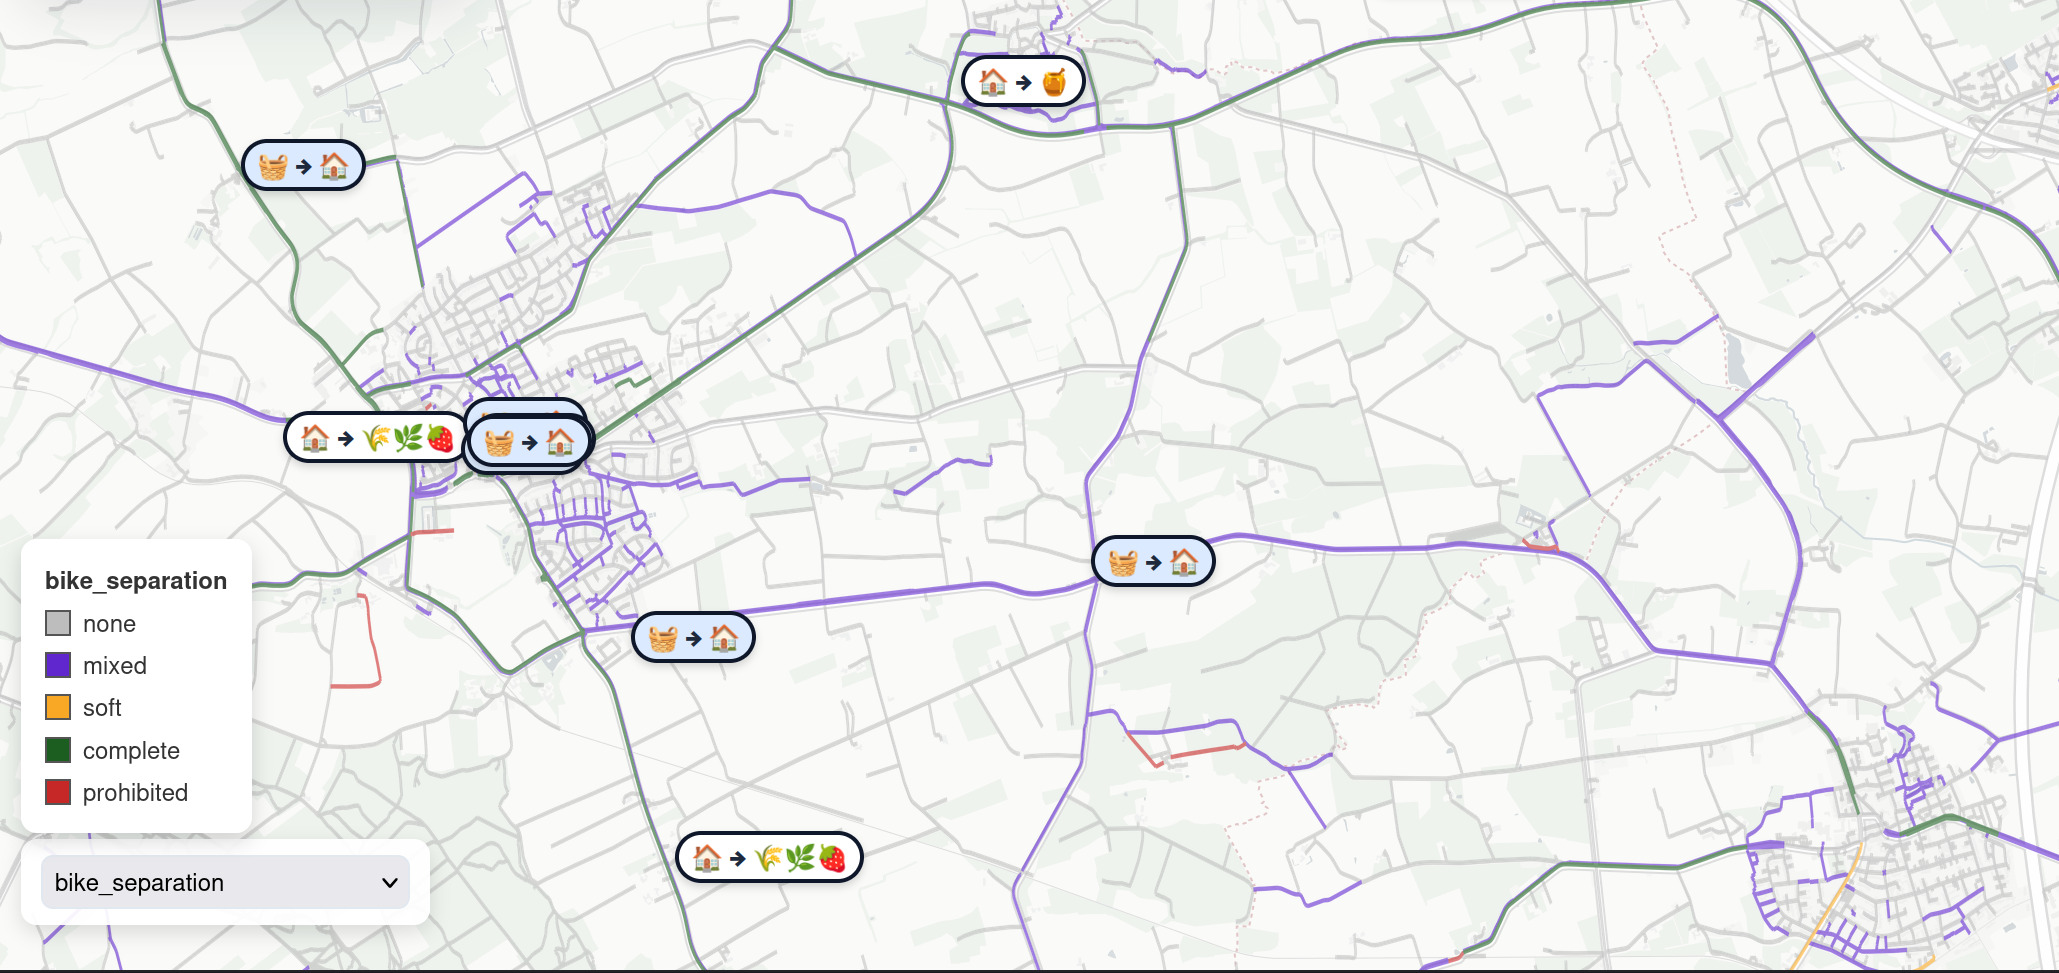
\includegraphics[width=0.75\textwidth]{figures/fig08_radinfrastruktur.jpg}
\caption[Radinfrastruktur in Havixbeck]{Radinfrastruktur in Havixbeck (eigene Darstellung, Datenquelle: \cite{OpenStreetMap}\interaktivekarte[Getrennte Radwege][raster=bike_separation])}
\label{fig:radinfrastruktur}
\end{figure}

Das ist aber nicht automatisch die beste Wahl: Oft führt die kürzere, vom Modell bevorzugte Radroute durch ruhige Wohnstraßen statt am Radweg der Umgehung, wie Bild~\ref{fig:routenvergleich2} zeigt. Das ist auch für die zukünftige Planung wichtig.

\begin{figure}[htbp]
\centering
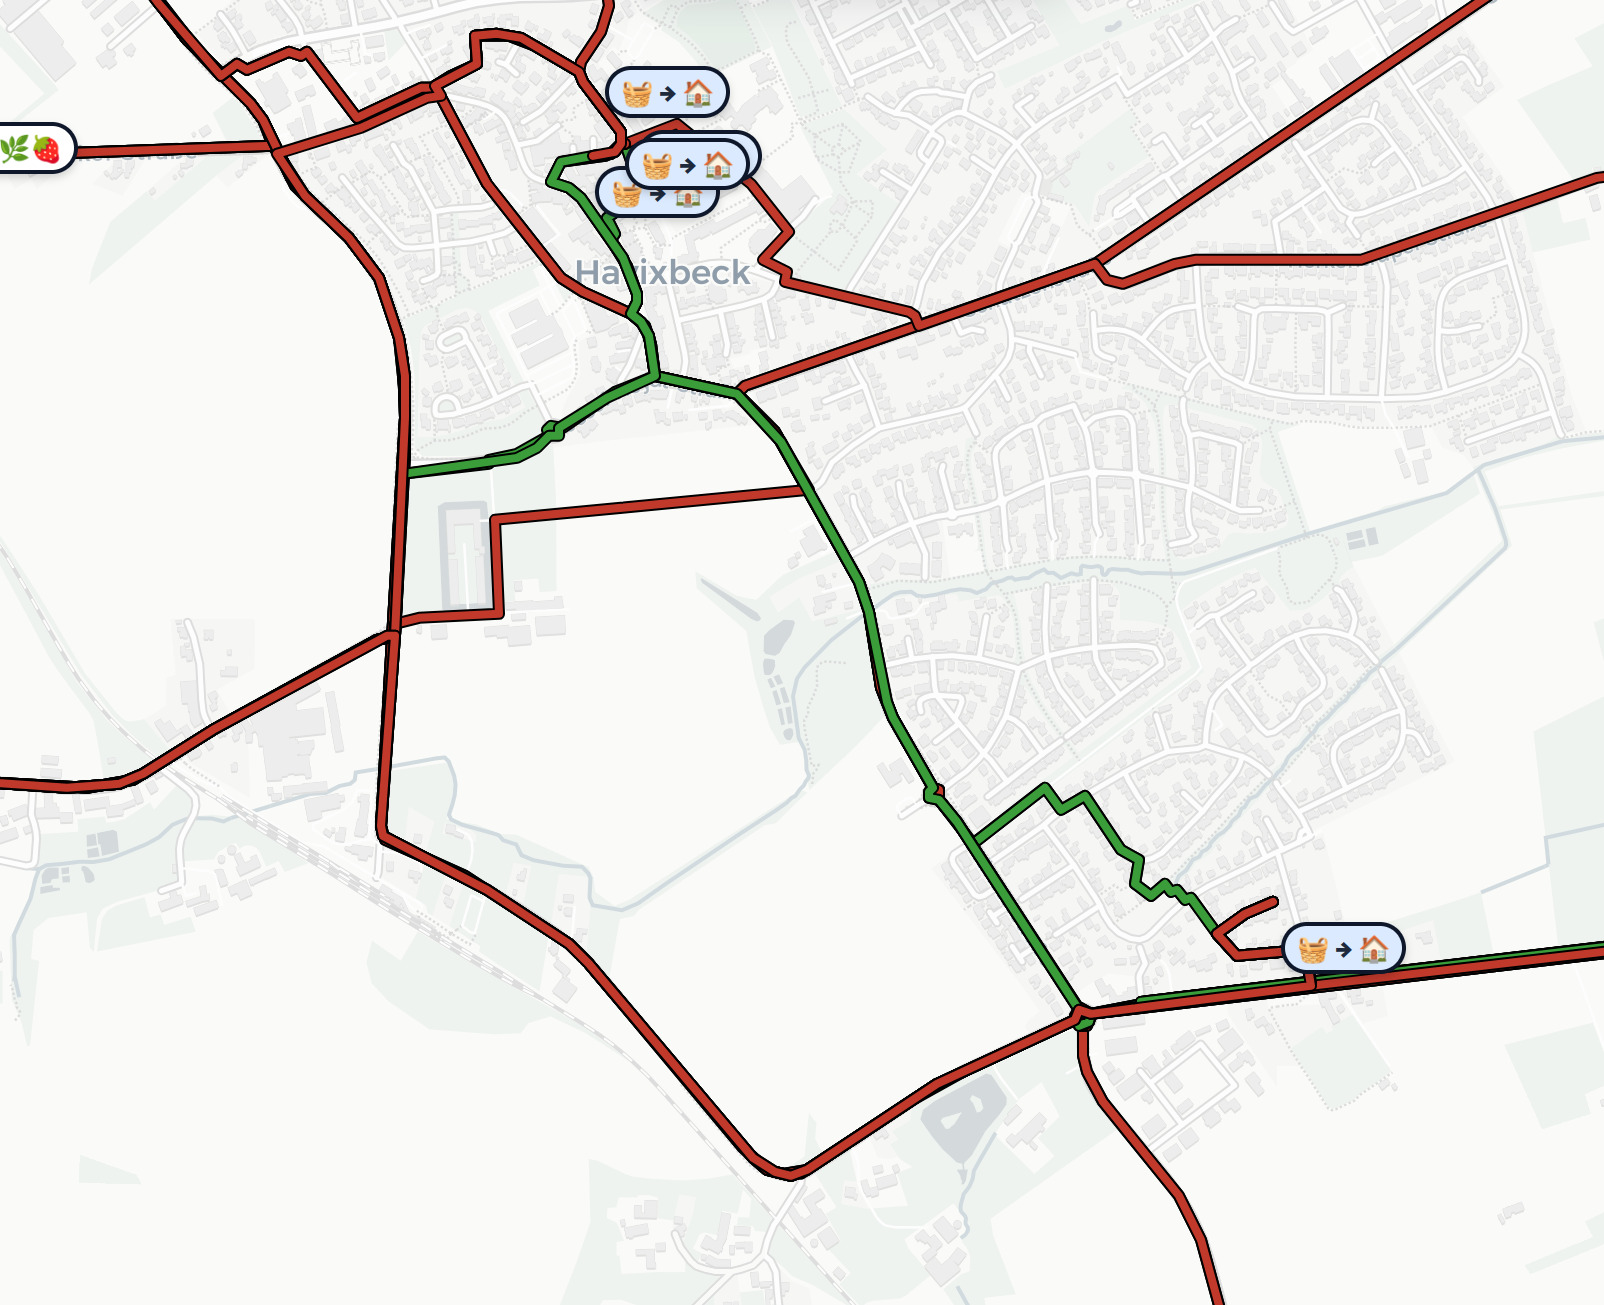
\includegraphics[width=0.55\textwidth]{figures/fig09_routenvergleich_ortskern.jpg}
\caption[Routenvergleich Ortskern]{Unterschiedliche Routen für Auto (rot) und Fahrrad (grün): Fahrradfahrende bevorzugen kürzere Wege durch den Ortskern, auch wenn entlang der Hauptstraßen separate Radwege vorhanden sind (eigene Darstellung, Datenquelle: \cite{OpenStreetMap}\interaktivekarte)}
\label{fig:routenvergleich2}
\end{figure}

\subsection{CO\textsubscript{2}-Modell}

Jede Kante bekommt eine CO\textsubscript{2}-Emission in g/km. Grundlage ist der HBEFA-Anwendungsleitfaden \parencite{Notter2025}, der Emissionen nach „Verkehrssituation“ klassifiziert: einer Kombination aus Gebietstyp (städtisch/außerorts), Straßentyp, zulässiger Geschwindigkeit und Level of Service (LOS, ein Maß für den Verkehrsfluss von A = freie Fahrt bis F = Stau). Die vollständige HBEFA-Datenbank mit exakten Emissionsfaktoren je Verkehrssituation ist kostenpflichtig und liegt dem Projekt nicht vor, nur der öffentliche Leitfaden mit den zugrunde liegenden Kurvenformen und Faktortabellen.

Das Projekt bildet die im Leitfaden beschriebene Systematik deshalb selbst nach, statt die Originaldaten zu verwenden: Für jede Kante wird zunächst eine geschwindigkeitsabhängige Basisemission berechnet, die anschließend mit einem Straßentyp-Faktor, einem LOS-Faktor und einem Steigungsfaktor multipliziert wird. Alle drei Faktoren sind nicht gemessen, sondern aus den Grafiken und Tabellen des öffentlichen Leitfadens abgelesen. Die Straßentyp-Faktoren liegen zwischen 0,95 und 1,40, je nachdem wie gleichmäßig der Verkehr auf diesem Straßentyp typischerweise fließt. Der LOS-Faktor wird für das gesamte Untersuchungsgebiet einheitlich als LOS~B angesetzt (Faktor 1,05), da Havixbeck und sein Umland ländlich geprägt sind und der Verkehr dort praktisch immer frei fließt (kein Stop-and-go wie in Städten).

Die Basisemission selbst ist ein Polynom zweiten Grades in der Geschwindigkeit $v$ (in km/h), für einen Benzin-Pkw beispielsweise

\begin{equation}
E_{\text{Basis}}(v) = 215 - 2{,}6\,v + 0{,}019\,v^{2}, \qquad v \text{ in km/h}, \quad E_{\text{Basis}} \text{ in g/km}
\end{equation}

Diese Kurve bildet die im Leitfaden gezeigte U-Form nach: Bei sehr niedriger Geschwindigkeit ist der Verbrauch pro Kilometer hoch, weil der Motor viel Zeit für wenig zurückgelegte Strecke braucht. Mit steigender Geschwindigkeit sinkt der Verbrauch bis zu einem Minimum im mittleren Geschwindigkeitsbereich. Bei hoher Geschwindigkeit steigt er durch den zunehmenden Luftwiderstand wieder an. Für Elektro-Lastenräder wird keine CO\textsubscript{2}-Emission angesetzt, da sie für diese Fahrten keine fossile Energie verbrauchen.

\section{Von Kanten-Scores zu Liefertouren: automatische und manuelle Schleifen}

Fahrzeiten und Scores werden zu einer Paarmatrix verdichtet, aus der die Tourenplanung je Akteur eine Lieferschleife bestimmt. Für das automatische Screening werden zwei Schleifentypen unterschieden: die Produzenten-Schleife (Anlieferung, 5-km-Radius) und die Konsumenten-Schleife (Abholung, Mindestabdeckung aller Produkte, ohne Radiusgrenze). Beide lösen ein Traveling-Salesman-Problem mit minimaler Fahrzeit \parencite{Applegate2006}, die Konsumenten-Variante als Covering-Salesman-Problem \parencite{Current1989}. Beide werden exakt gelöst, mit einer selbst implementierten Held-Karp-Bitmask-Dynamic-Programming-Lösung (reines Python/NumPy, ohne externen Solver wie OR-Tools) statt einer Heuristik. Die dabei auftretende Anzahl an Halten pro Schleife bleibt klein genug (deutlich unter 15), sodass die exponentielle Laufzeit der exakten Lösung praktisch unproblematisch ist.

Die manuellen Szenarien sind anhand von Interview-Daten als feste Stopp-Abfolge definiert. Beide Schleifentypen, automatisch und manuell, bilden zusammen die Grundlage für die konkreten Konzeptauswertungen in Kapitel~\ref{ch:massnahmen}.

\section{Kartendarstellung}

Alle im Rahmen dieser Arbeit berechneten Routen lassen sich zusätzlich in einer interaktiven Karte einsehen und erkunden. Das gilt sowohl für die automatischen Produzenten- und Konsumenten-Schleifen als auch für die manuell definierten Konzeptszenarien: \url{https://miguelurenapliego.github.io/RadlogistikHavixbeck}

\chapter{Maßnahmen / Konzept}
\label{ch:massnahmen}

Durch die in Kapitel~\ref{ch:auswahl} betrachteten Akteure ergeben sich mehrere Konzepte, welche im Folgenden vorgestellt und mit den in Kapitel~\ref{ch:routing} berechneten Routenscores ausgewertet werden. Alle angegebenen Werte sind vollständige Rundtouren (Hin- und Rückweg). Jede Schleife wird regelmäßig gefahren, konsistent mit den Interviews, in denen die Betriebe durchweg ein geringes Güteraufkommen angaben.

\section{Konzept 1: Stift Tilbeck}

Für das Stift Tilbeck bietet sich der Einsatz eines betriebseigenen E-Lastenrads als nachhaltige Alternative zur aktuellen Transportlösung an. Derzeit wird der Verkaufsstand für den Havixbecker Wochenmarkt mit einem Pkw-Anhänger transportiert. Durch ein Lastenrad könnte dieser motorisierte Transport auf den kurzen Strecken ersetzt werden.

Ein betriebseigenes Lastenrad ist gegenüber einem Sharing-System geeigneter, da auf dem Gelände des Stifts sichere Abstellmöglichkeiten sowie Ladeinfrastruktur vorhanden sind. Dadurch ist das Fahrzeug dauerhaft verfügbar und flexibel einsetzbar.

Das Haupteinsatzgebiet liegt in der Belieferung des etwa fünf Kilometer entfernten Wochenmarkts in Havixbeck. Auch die gelegentliche Belieferung des benachbarten Restaurants „Das Lauschig“ kann mit dem Lastenrad erfolgen. Zusätzlich soll das Fahrzeug als mobile Verkaufseinheit dienen. Hierfür notwendige Anpassungen können durch die vorhandenen technischen Möglichkeiten und Mitarbeitenden des Stifts selbst umgesetzt werden.

Durch die individuelle Gestaltung kann das Lastenrad die Identifikation mit dem Stift Tilbeck stärken und als sichtbares Zeichen für nachhaltige Mobilität dienen. Gleichzeitig besitzt es das Potenzial, die Akzeptanz von Radlogistik im ländlichen Raum zu fördern.

In einem Gespräch bewertete der Fachbereichsleiter der Produktion, Herr Claus Tenbrink, eine Umstellung auf Radlogistik positiv. Während er andere Produktionsbereiche aufgrund von Transportentfernungen sowie Größe und Gewicht der Waren ausschloss, sah er insbesondere im Gärtnereibetrieb geeignete Einsatzmöglichkeiten. Zusätzlich wurde eine Verlagerung einzelner Personenbeförderungen auf den Radverkehr angeregt, die aufgrund fehlender B2B-Logistik in dieser Arbeit jedoch nicht betrachtet wird.

Als mögliches Grundmodell wird ein Lastenrad nach dem Berliner Modell vorgeschlagen, wie in Bild~\ref{fig:berliner-lastenrad} dargestellt. Vorteile sind der sichere Stand durch die Mehrspurigkeit sowie das geringe Gewicht, wodurch Beladung, Verkauf und Rangieren erleichtert werden. Ein solches Lastenrad kostet etwa 3.400\,€ ohne und 6.200\,€ mit Elektroantrieb \parencite{Pedalpower2025}.

\begin{figure}[htbp]
\centering
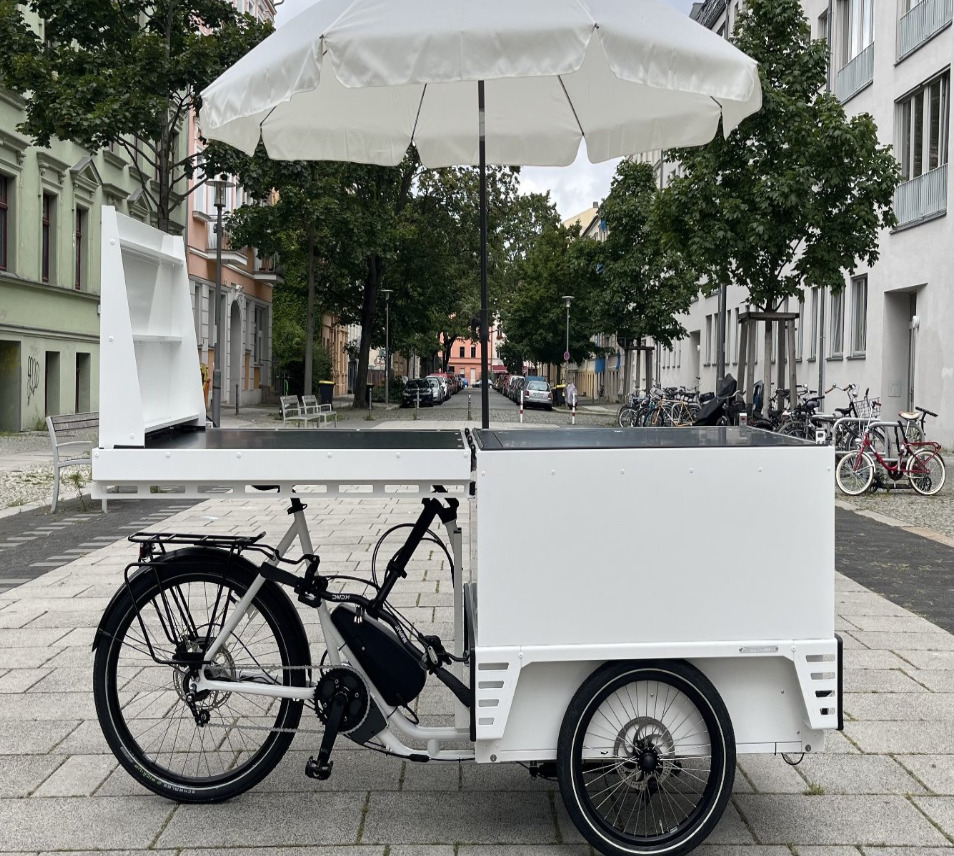
\includegraphics[width=0.6\textwidth]{figures/fig16_berliner_lastenrad.jpg}
\caption[Lastenrad nach dem Berliner Modell]{Lastenrad nach dem Berliner Modell mit Aufbau als mobiler Verkaufsstand (Bildquelle: \cite{PedalpowerND})}
\label{fig:berliner-lastenrad}
\end{figure}

Die Routing-Auswertung der in Bild~\ref{fig:konzept-stift} dargestellten Schleife Stift Tilbeck, Wochenmarkt und „Das Lauschig“ bestätigt den positiven Eindruck aus dem Gespräch mit Herrn Tenbrink, wie Tabelle~\ref{tab:stift-route} zeigt:

\begin{figure}[htbp]
\centering
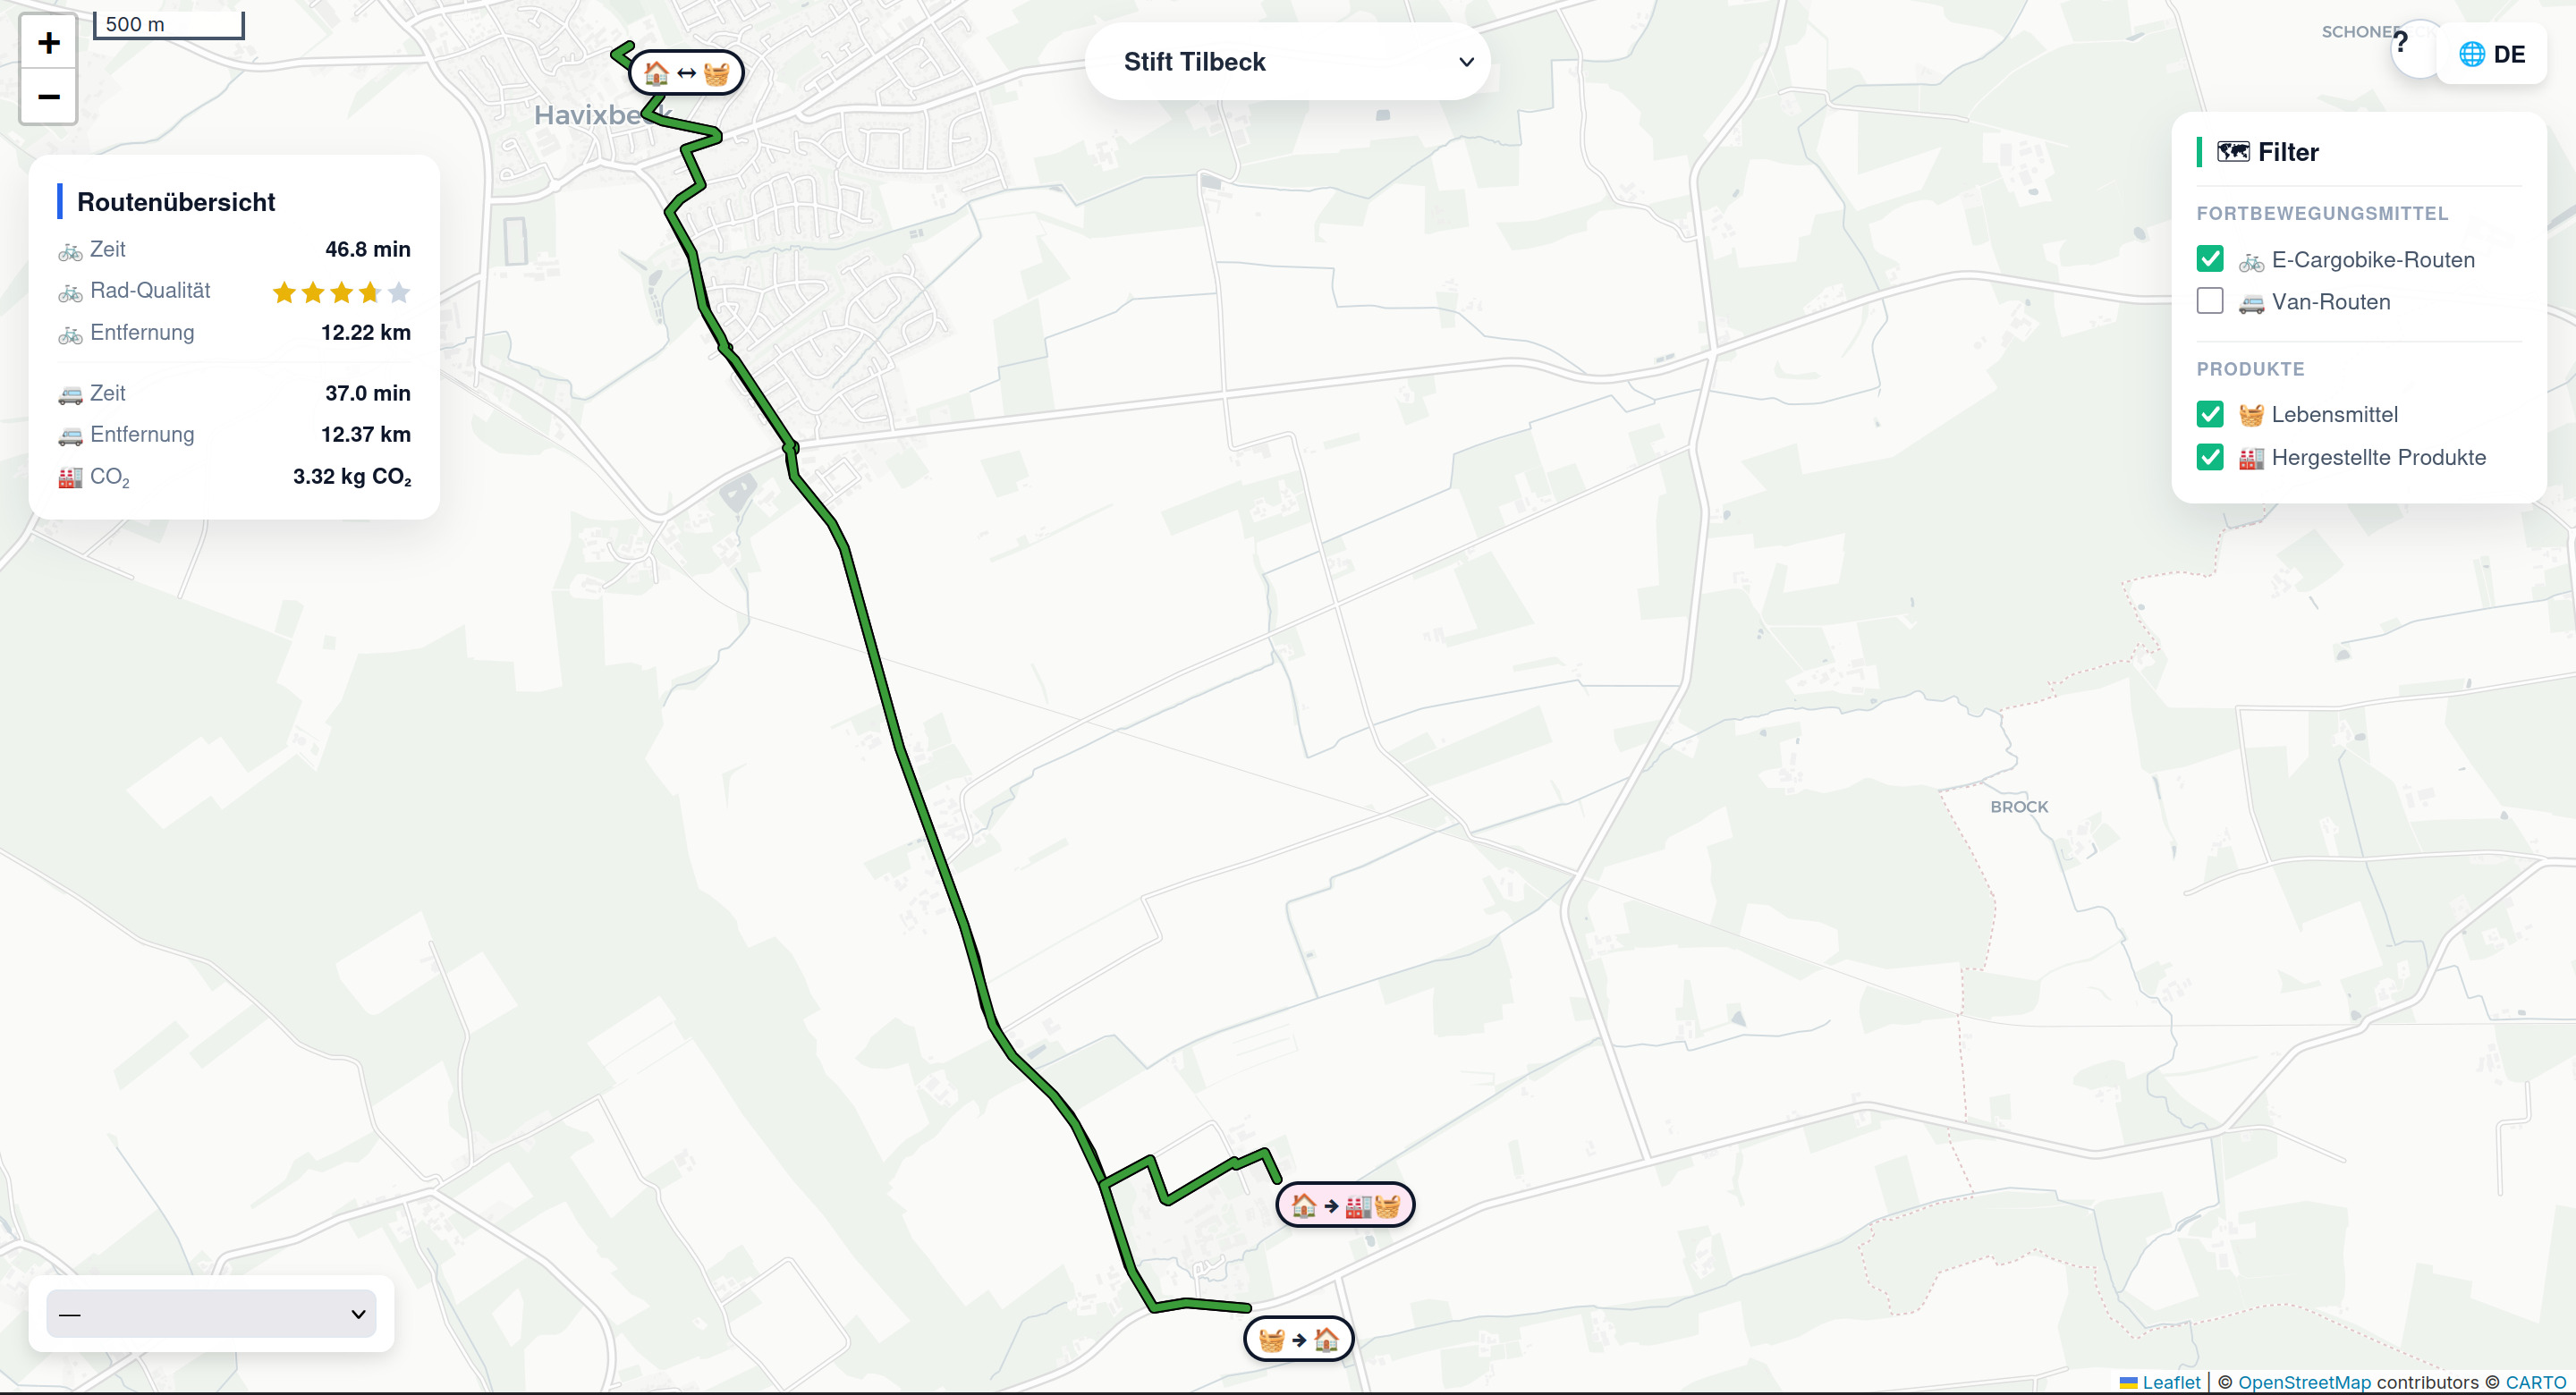
\includegraphics[width=0.85\textwidth]{figures/fig14_konzept_stift_tilbeck.jpg}
\caption[Radlogistikkonzept für das Stift Tilbeck]{Radlogistikkonzept für das Stift Tilbeck (eigene Darstellung, Datenquelle: \cite{OpenStreetMap}\interaktivekarte[Stift Tilbeck][layer=custom_2])}
\label{fig:konzept-stift}
\end{figure}

{\small
\begin{longtable}{@{}lrrrrrrr@{}}
\caption{Radlogistikroute für das Stift Tilbeck}\label{tab:stift-route}\\
\toprule
\textbf{Standort} & \textbf{Pkw min} & \textbf{Pkw km} & \textbf{Pkw CO\textsubscript{2} kg} & \textbf{Rad min} & \textbf{Rad km} & \textbf{Mehrzeit \%} & \textbf{Score} \\
\midrule
\endfirsthead
\multicolumn{8}{@{}l}{\small\itshape Fortsetzung von der vorherigen Seite}\\
\toprule
\textbf{Standort} & \textbf{Pkw min} & \textbf{Pkw km} & \textbf{Pkw CO\textsubscript{2} kg} & \textbf{Rad min} & \textbf{Rad km} & \textbf{Mehrzeit \%} & \textbf{Score} \\
\midrule
\endhead
\midrule
\multicolumn{8}{@{}r}{\small\itshape Fortsetzung auf der nächsten Seite}\\
\endfoot
\bottomrule
\endlastfoot
Alexianer Stift Tilbeck & 37,0 & 12,37 & 3,32 & 46,8 & 12,22 & 26,6 & 8,0 \\
\end{longtable}
}

Mit einem Bike-Score von 8,0 erreicht diese Schleife den besten Wert aller drei Konzepte. Auch wirtschaftlich ist der Umstieg attraktiv: Die Kosten eines Lastenrads nach dem Berliner Modell (3.400--6.200\,€, \cite{PedalpowerND}) liegen in einer ähnlichen Größenordnung wie die eines neuwertigen Pkw mit vergleichbarer Nutzung als mobiler Verkaufsstand. Zusätzlich unterliegt der Umbau eines Lastenrads zum Verkaufsstand deutlich weniger regulatorischen Anforderungen (z.\,B. keine Fahrzeugzulassung, keine Hauptuntersuchung) als der eines Pkw, was den Aufbau vereinfacht und zusätzlich kostengünstiger macht. Unter den drei Konzepten hat Stift Tilbeck damit das größte Potenzial für eine kurzfristige Umsetzung.

\section{Konzept 2: Lieferungen von Landwirtschaftsbetrieben zu Gastronomien}

Das zweite Konzept betrachtet die Lieferbeziehungen zwischen landwirtschaftlichen Betrieben im Umland und Gastronomiebetrieben in Havixbeck. Dabei werden regionale Produkte direkt von den Höfen zu den Abnehmern transportiert.

Wie bei Konzept 1 wird der Einsatz betriebseigener Lastenräder vorgesehen. Ein zentrales Sharing-System ist aufgrund der Entfernungen zwischen Höfen und Ortskern sowie der parallelen Nutzung durch Wochenmarktbelieferungen keine geeignete Lösung. Die Lagerung und Beladung der Fahrzeuge auf den Betriebsgeländen ermöglicht hingegen eine flexible Nutzung ohne zusätzliche Infrastruktur.

Als geeignetes Fahrzeug wird der in Bild~\ref{fig:carlacargo-anhaenger} gezeigte Carla-Cargo-Lastenanhänger vorgeschlagen. Durch seine mehrspurige Bauweise ermöglicht er ein sicheres Be- und Entladen. Zudem kann der Anhänger vom Zugfahrrad getrennt werden, wodurch das Fahrrad unabhängig für weitere betriebliche Fahrten genutzt werden kann. Dies erhöht die Flexibilität und Akzeptanz des Systems.

\begin{figure}[htbp]
\centering
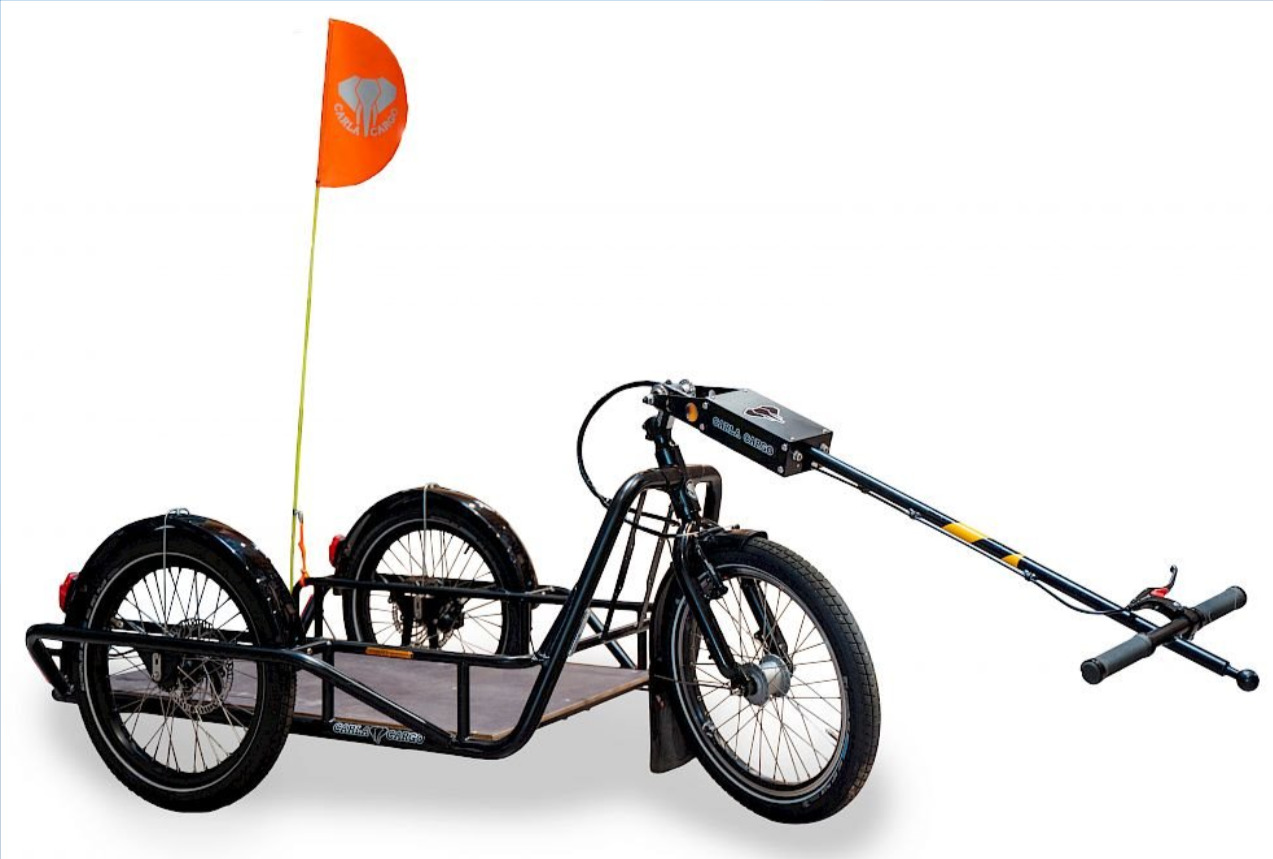
\includegraphics[width=0.6\textwidth]{figures/fig15_carlacargo_anhaenger.jpg}
\caption[Carla-Cargo-Lastenanhänger]{Carla-Cargo-Lastenanhänger (Bildquelle: \cite{CarlaCargo})}
\label{fig:carlacargo-anhaenger}
\end{figure}

Da die Lieferungen überwiegend saisonal erfolgen, kann der Anhänger außerhalb der Saison eingelagert werden. Die nicht motorisierte Variante mit Bremsunterstützung kostet etwa 3.500\,€ und kann mit vorhandenen Pedelecs kombiniert werden. Alternativ besteht die Möglichkeit eines elektrisch unterstützten Modells für etwa 6.500\,€, welches zusätzlich eine Schiebehilfe für das Rangieren schwerer Lasten bietet \parencite{CarlaCargo}.

Die Eignung des Konzepts hängt stark von der Lage der einzelnen Betriebe ab, wie die Auswertung der Erzeuger-Schleife in Bild~\ref{fig:anliefer-landwirtschaft} und Tabelle~\ref{tab:landwirtschaft} zeigt. Die Einrichtung eines Mikro-Hubs im Ortszentrum von Havixbeck wird nicht empfohlen, da die Gastronomiebetriebe überwiegend zentral am Marktplatz liegen und eine direkte Belieferung effizienter ist.

\begin{figure}[htbp]
\centering
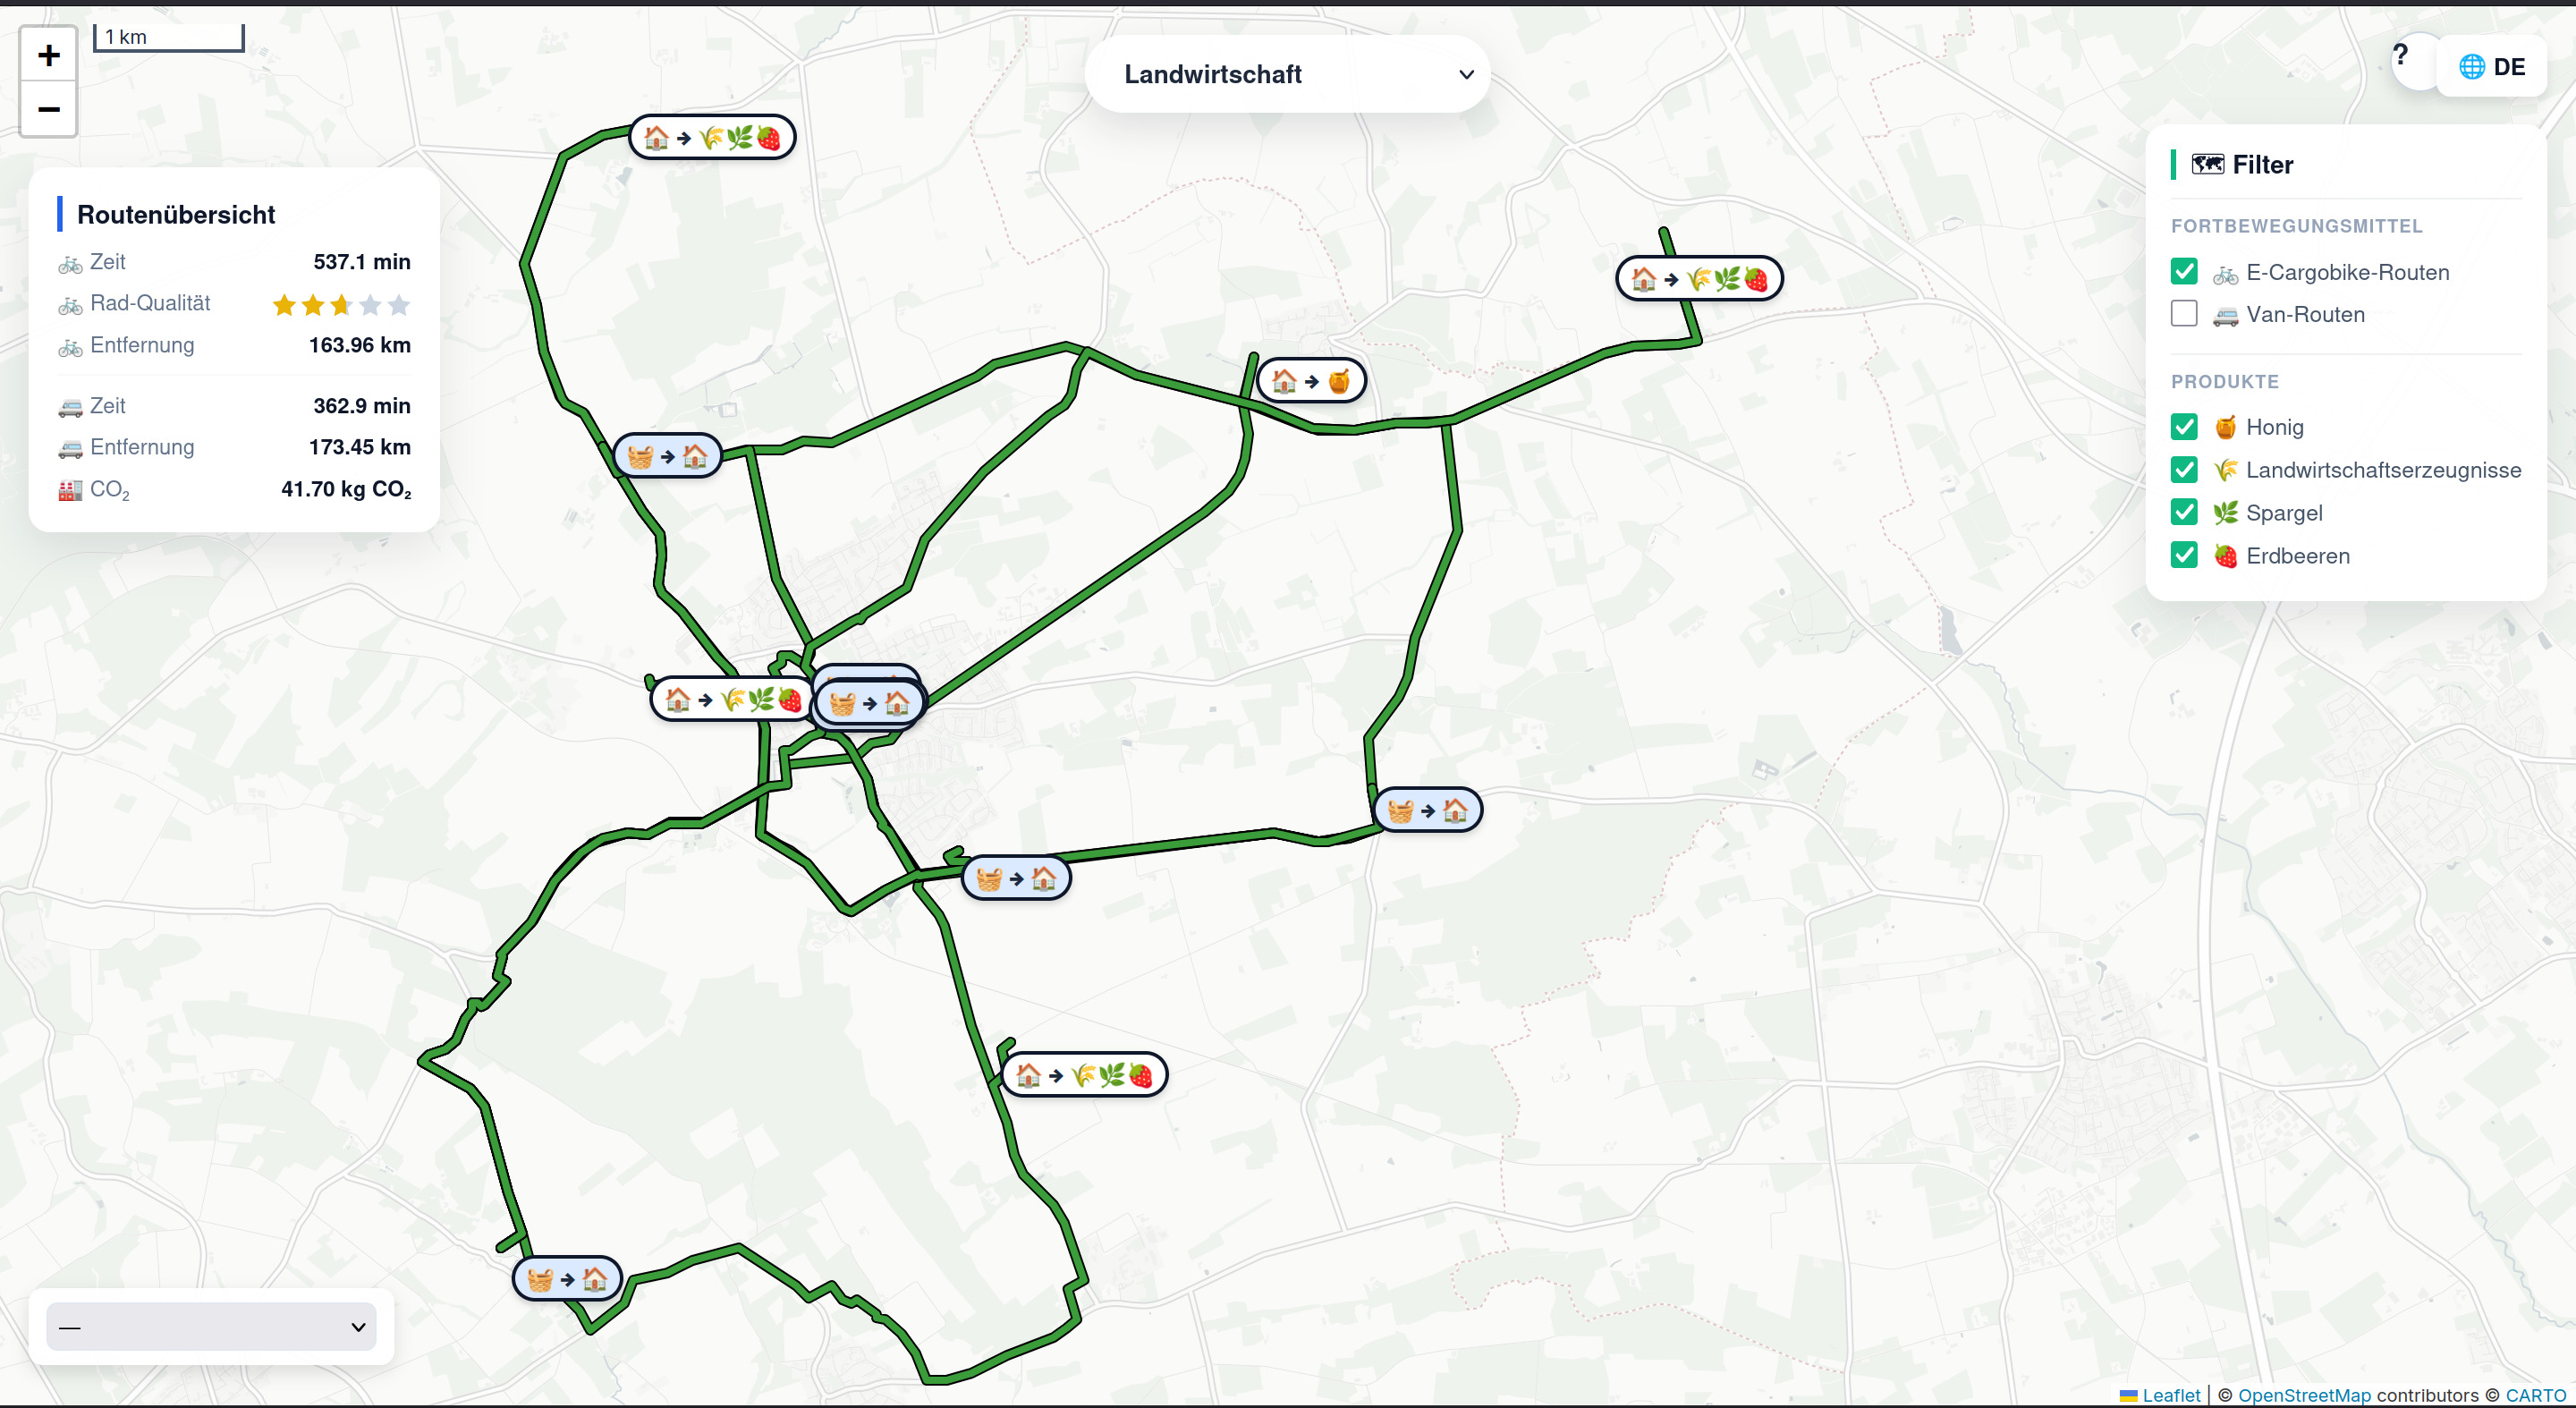
\includegraphics[width=0.85\textwidth]{figures/fig12_anliefermodell_landwirtschaft.jpg}
\caption[Anliefermodell aus lokaler Landwirtschaft]{Variante mit einem Anliefermodell für Restaurants komplett aus lokaler Landwirtschaft (eigene Darstellung, Datenquelle: \cite{OpenStreetMap}\interaktivekarte[Landwirtschaft][layer=custom_0])}
\label{fig:anliefer-landwirtschaft}
\end{figure}

{\small
\begin{longtable}{@{}lrrrrrrr@{}}
\caption{Routen für landwirtschaftliche Betriebe}\label{tab:landwirtschaft}\\
\toprule
\textbf{Standort} & \textbf{Pkw min} & \textbf{Pkw km} & \textbf{Pkw CO\textsubscript{2} kg} & \textbf{Rad min} & \textbf{Rad km} & \textbf{Mehrzeit \%} & \textbf{Score} \\
\midrule
\endfirsthead
\multicolumn{8}{@{}l}{\small\itshape Fortsetzung von der vorherigen Seite}\\
\toprule
\textbf{Standort} & \textbf{Pkw min} & \textbf{Pkw km} & \textbf{Pkw CO\textsubscript{2} kg} & \textbf{Rad min} & \textbf{Rad km} & \textbf{Mehrzeit \%} & \textbf{Score} \\
\midrule
\endhead
\midrule
\multicolumn{8}{@{}r}{\small\itshape Fortsetzung auf der nächsten Seite}\\
\endfoot
\bottomrule
\endlastfoot
Hof Richter       & 60,7  & 28,91 & 6,96  & 89,5  & 26,47 & 47,4 & 5,7 \\
Franz Himker      & 71,7  & 33,27 & 8,16  & 105,6 & 32,51 & 47,3 & 6,4 \\
Hof Heilers-Lülf  & 68,4  & 32,91 & 7,83  & 100,6 & 30,47 & 47,1 & 5,8 \\
Imkerei Gerdes    & 74,3  & 35,60 & 8,60  & 109,3 & 34,06 & 47,1 & 6,7 \\
Hof Baumeister    & 87,8  & 42,75 & 10,15 & 132,1 & 40,46 & 50,5 & 6,1 \\
\midrule
\textbf{Summe} & \textbf{362,9} & \textbf{173,45} & \textbf{41,70} & \textbf{537,1} & \textbf{163,96} & -- & -- \\
\textbf{Durchschnitt (Ø)} & -- & -- & -- & -- & -- & \textbf{47,9} & \textbf{6,1} \\
\end{longtable}
}

Restaurants beziehen aktuell kaum lokale Produkte. Das Konzept erkundet, was möglich wäre, wenn sie es täten. Der absolute Zeitunterschied liegt bei fünf der sechs Betriebe über 30 Minuten. Der Pkw lässt sich dadurch aber nicht komplett ersetzen: Gut die Hälfte der Restaurants liegt nicht im Ortskern, sondern verstreut über die gesamte Gemeinde. Ohne eine höhere Zeittoleranz der Betriebe ist Radlogistik als vollständiger Ersatz des Pkw nicht möglich. Für Lieferungen nach Münster oder andere weiter entfernte Städte bleibt der Pkw ohnehin unverzichtbar.

\subsection{Direkte Anbindung an den Wochenmarkt}

Statt der vollen Rundtour lohnt sich auch der Blick auf den Wochenmarkt als gemeinsamen Treffpunkt: Sowohl Landwirtschaftsbetriebe als auch Restaurants können dort direkt anfahren, um zu verkaufen oder einzukaufen (Bild~\ref{fig:wochenmarkt-zentral}). Auf dieser einzelnen Strecke sind Bike-Score und Rad-Mehrzeit deutlich besser als auf der vollen Rundtour, wie Tabelle~\ref{tab:wochenmarkt} zeigt. Hier ist Radlogistik sehr konkurrenzfähig gegenüber dem Pkw.

\begin{figure}[htbp]
\centering
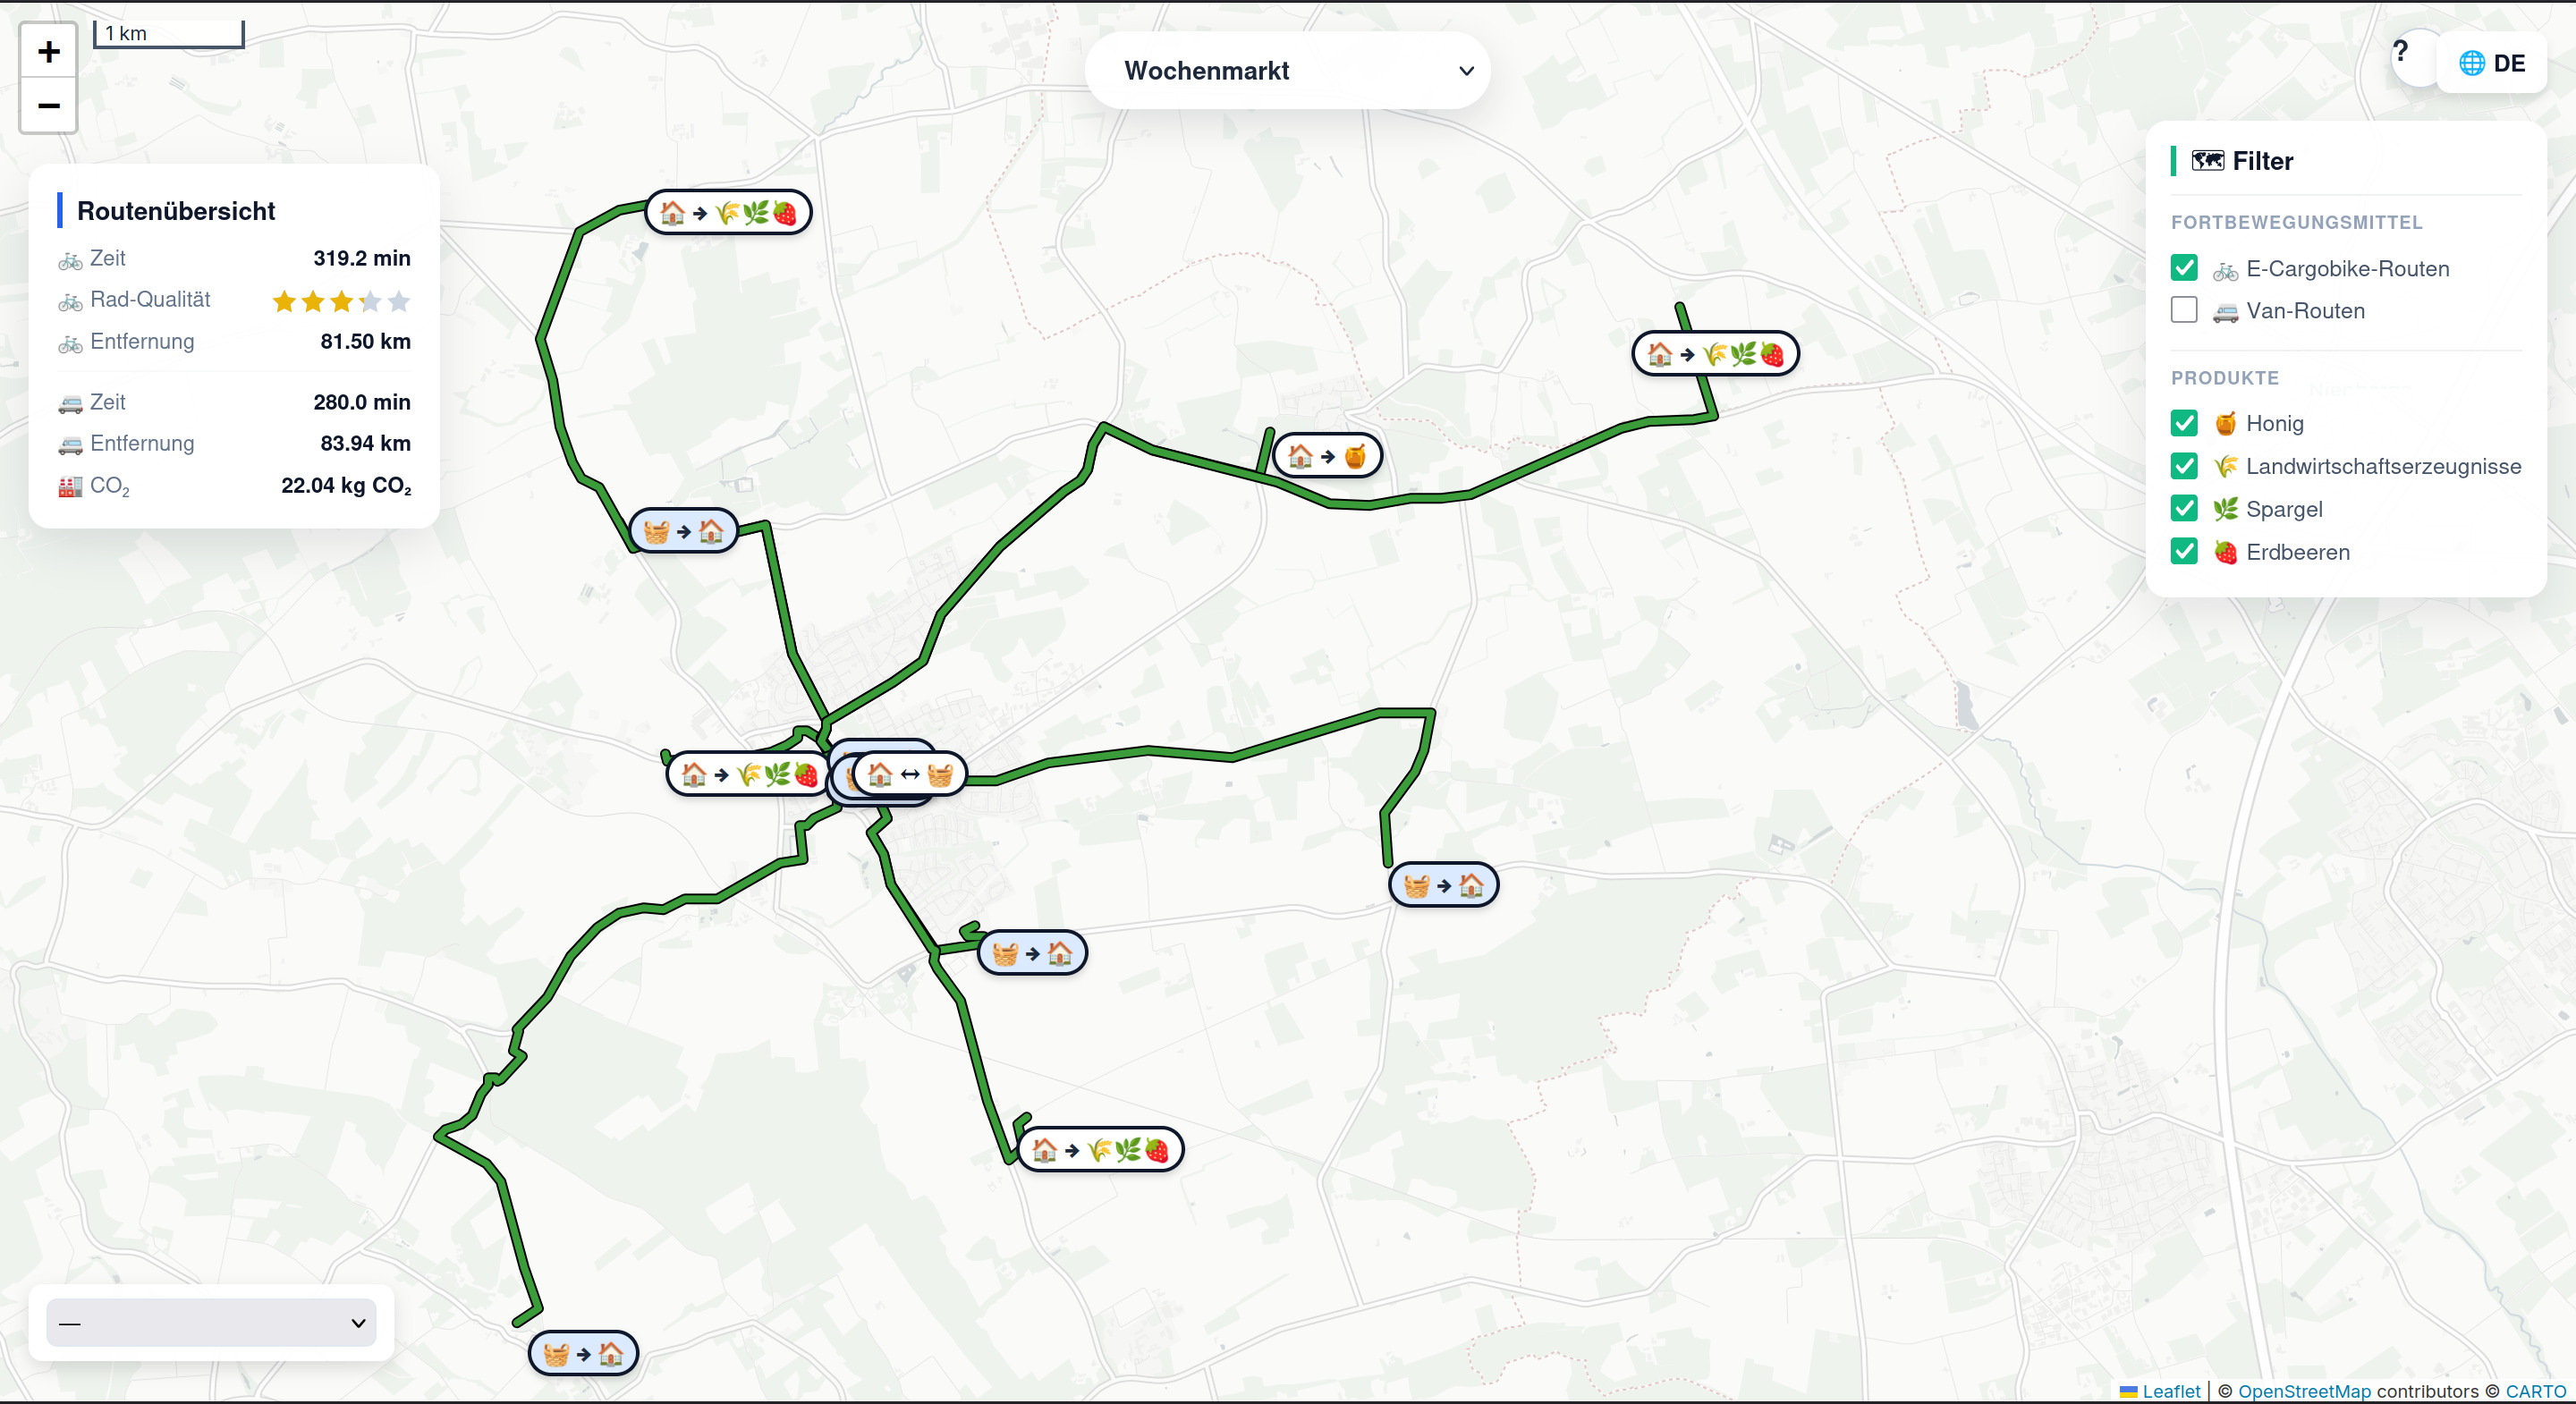
\includegraphics[width=0.85\textwidth]{figures/fig13_wochenmarkt_zentral.jpg}
\caption[Wochenmarkt als zentraler Logistikpunkt]{Variante mit Wochenmarkt als zentralem Logistikpunkt für Restaurants und lokale Betriebe (eigene Darstellung, Datenquelle: \cite{OpenStreetMap}\interaktivekarte[Wochenmarkt][layer=custom_1])}
\label{fig:wochenmarkt-zentral}
\end{figure}

{\small
\begin{longtable}{@{}lrrrrrrr@{}}
\caption{Routen für Restaurants und landwirtschaftliche Betriebe zum Wochenmarkt}\label{tab:wochenmarkt}\\
\toprule
\textbf{Standort} & \textbf{Pkw min} & \textbf{Pkw km} & \textbf{Pkw CO\textsubscript{2} kg} & \textbf{Rad min} & \textbf{Rad km} & \textbf{Mehrzeit \%} & \textbf{Score} \\
\midrule
\endfirsthead
\multicolumn{8}{@{}l}{\small\itshape Fortsetzung von der vorherigen Seite}\\
\toprule
\textbf{Standort} & \textbf{Pkw min} & \textbf{Pkw km} & \textbf{Pkw CO\textsubscript{2} kg} & \textbf{Rad min} & \textbf{Rad km} & \textbf{Mehrzeit \%} & \textbf{Score} \\
\midrule
\endhead
\midrule
\multicolumn{8}{@{}r}{\small\itshape Fortsetzung auf der nächsten Seite}\\
\endfoot
\bottomrule
\endlastfoot
Yosara            & 8,2  & 0,33  & 0,19 & 4,0  & 0,33  & $-51,1$ & 3,1 \\
Gasthaus Kemper   & 8,2  & 0,33  & 0,19 & 4,0  & 0,33  & $-51,1$ & 3,1 \\
Apollon           & 8,6  & 0,43  & 0,22 & 4,5  & 0,43  & $-47,6$ & 3,7 \\
Wanjas            & 9,0  & 0,58  & 0,26 & 5,0  & 0,58  & $-44,3$ & 4,2 \\
Brauhaus Klute    & 20,9 & 5,37  & 1,55 & 22,4 & 5,77  & 7,1  & 8,2 \\
Hof Richter       & 15,0 & 2,92  & 0,85 & 16,4 & 2,92  & 9,3  & 7,2 \\
Haus Füsting      & 24,2 & 5,17  & 1,67 & 28,1 & 4,69  & 15,9 & 6,6 \\
Franz Himker      & 26,2 & 7,56  & 2,10 & 31,3 & 7,40  & 19,4 & 8,1 \\
Gasthaus Stevertal& 36,2 & 14,33 & 3,50 & 44,5 & 12,04 & 23,0 & 3,6 \\
Hof Heilers-Lülf  & 29,9 & 12,10 & 2,77 & 36,9 & 10,97 & 23,5 & 7,0 \\
Imkerei Gerdes    & 25,3 & 8,52  & 2,21 & 31,6 & 9,12  & 25,1 & 9,4 \\
Landg.\ Overwaul  & 28,5 & 10,59 & 2,62 & 37,6 & 10,61 & 31,7 & 1,5 \\
Hof Baumeister    & 39,9 & 15,71 & 3,90 & 52,9 & 16,31 & 32,8 & 8,6 \\
\midrule
\textbf{Summe} & \textbf{280,0} & \textbf{83,94} & \textbf{22,04} & \textbf{319,2} & \textbf{81,50} & -- & -- \\
\textbf{Durchschnitt (Ø)} & -- & -- & -- & -- & -- & \textbf{$-0,5$} & \textbf{5,7} \\
\end{longtable}
}

Die vier zentrumsnahen Restaurants (Yosara, Kemper, Apollon, Wanjas) sind so nah am Wochenmarkt, dass die Radroute sogar schneller ist als die Pkw-Route: Trotz der kurzen Distanz fällt die Pkw-Fahrzeit hier überdurchschnittlich hoch aus, da der Ortskern rund um den Marktplatz weitgehend fußgängerzonenartig gestaltet ist und der Pkw dadurch nur mit stark reduzierter Geschwindigkeit durchfahren kann. Zusammen mit Brauhaus Klute, Hof Richter, Haus Füsting, Franz Himker, Gasthaus Stevertal und Hof Heilers-Lülf bleibt die Mehrzeit für 10 der 13 Ziele unter 25\,\%, deutlich besser als auf der jeweils vollen Rundtour. Die gesamte lokale Logistik durch Lastenräder zu ersetzen ist schwierig, die Wege zum Wochenmarkt dagegen leichter. Ein Lastenrad als Verkaufsstand, wie bei Stift Tilbeck, ließe sich auf weitere Höfe und Restaurants übertragen und Platz-/Verkehrsprobleme am Wochenmarkt entschärfen.

\section{Konzept 3: Abhollogistik von Gastronomien bei den Landwirtschaftsbetrieben}

Konzept 3 basiert auf den in Konzept 2 beschriebenen Lieferbeziehungen zwischen landwirtschaftlichen Betrieben und Gastronomien. Im Unterschied dazu übernehmen die Gastronomiebetriebe selbst die Abholung der Produkte von den Höfen. Hierfür wird ein Sharing-System für Lastenräder vorgeschlagen.

Das System sieht einen zentralen Abstellort im Ortskern von Havixbeck in direkter Nähe zu den Gastronomiebetrieben vor (s. Bild~\ref{fig:restaurants-landwirtschaft}). Da dort bereits eine Pedelec-Ladesäule vorhanden ist, kann die notwendige Infrastruktur mit geringem Aufwand ergänzt werden. Zum Schutz des Lastenrads wird eine abschließbare Fahrradbox empfohlen.

Die Reservierung kann zunächst per E-Mail erfolgen, während der Zugangsschlüssel über das nahegelegene Rathaus ausgegeben wird. Bei erfolgreicher Umsetzung kann das System durch digitale Zugangslösungen wie Schlüsseltresore oder QR-Codes erweitert werden.

Ein Vorteil des Konzepts liegt darin, dass die Gastronomiebetriebe keine eigenen Lastenräder anschaffen müssen und somit geringe Investitionskosten entstehen. Zusätzlich könnte das Fahrzeug grundsätzlich außerhalb der B2B-Nutzung Privatpersonen zur Verfügung gestellt werden, was jedoch nicht Bestandteil dieser Arbeit ist.

Als Fahrzeug wird ein einspuriges Lastenrad des Typs „Long John“ vorgeschlagen, wie in Bild~\ref{fig:long-john} gezeigt. Die große Transportbox ermöglicht den flexiblen Transport verschiedener Waren, während das ähnliche Fahrverhalten zu herkömmlichen Fahrrädern die Nutzung erleichtert. Die Kosten liegen bei etwa 6.800\,€ \parencite{mycargobike}.

\begin{figure}[htbp]
\centering
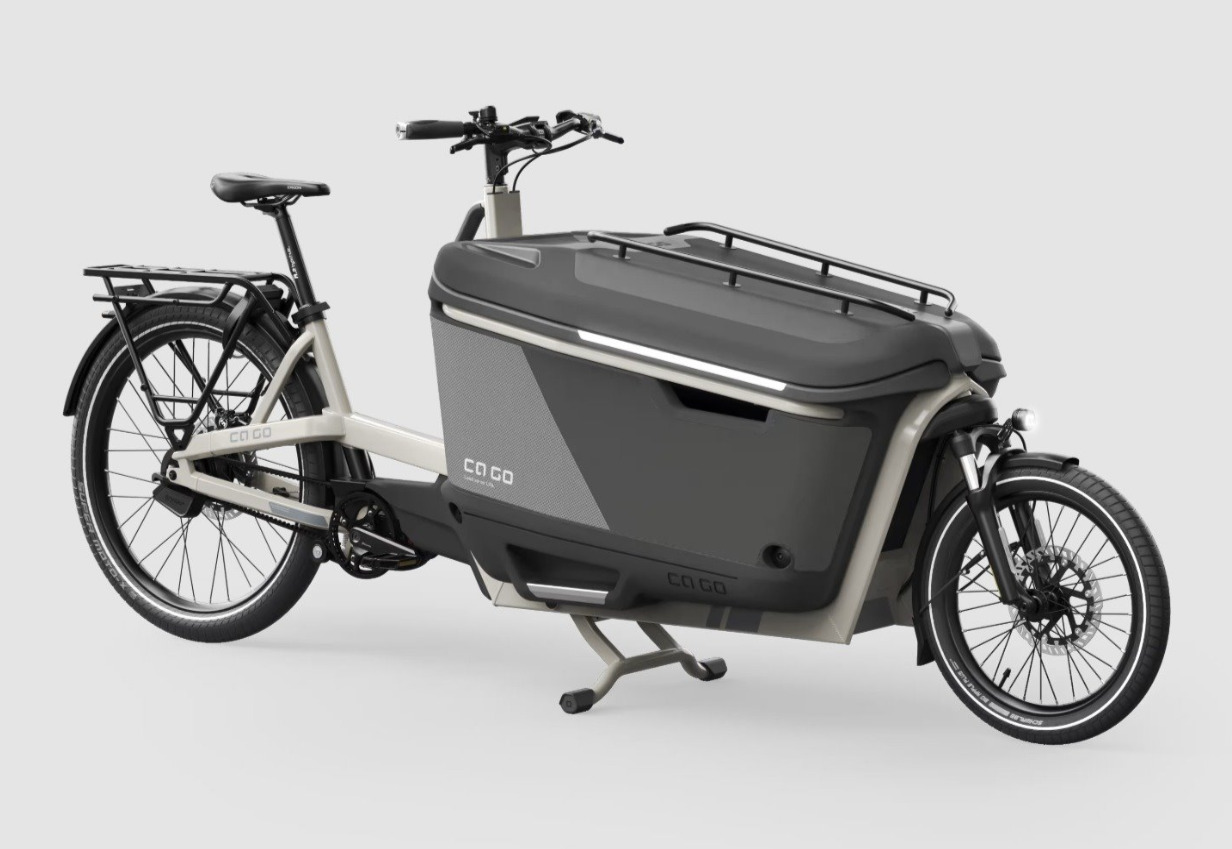
\includegraphics[width=0.6\textwidth]{figures/fig17_long_john.jpg}
\caption[Lastenrad des Typs Long John]{Lastenrad des Typs Long John (Bildquelle: \cite{mycargobike})}
\label{fig:long-john}
\end{figure}

Durch die Verlagerung der Transportverantwortung auf die Gastronomiebetriebe entstehen im Vergleich zu Konzept 2 veränderte Verkehrsströme. Um dieses Sharing-Konzept zu bewerten, wurden zwei Varianten geprüft: Restaurants holen selbst ab, oder Lebensmittelbetriebe liefern direkt.

\subsection{Restaurants (Abholung)}

\begin{figure}[htbp]
\centering
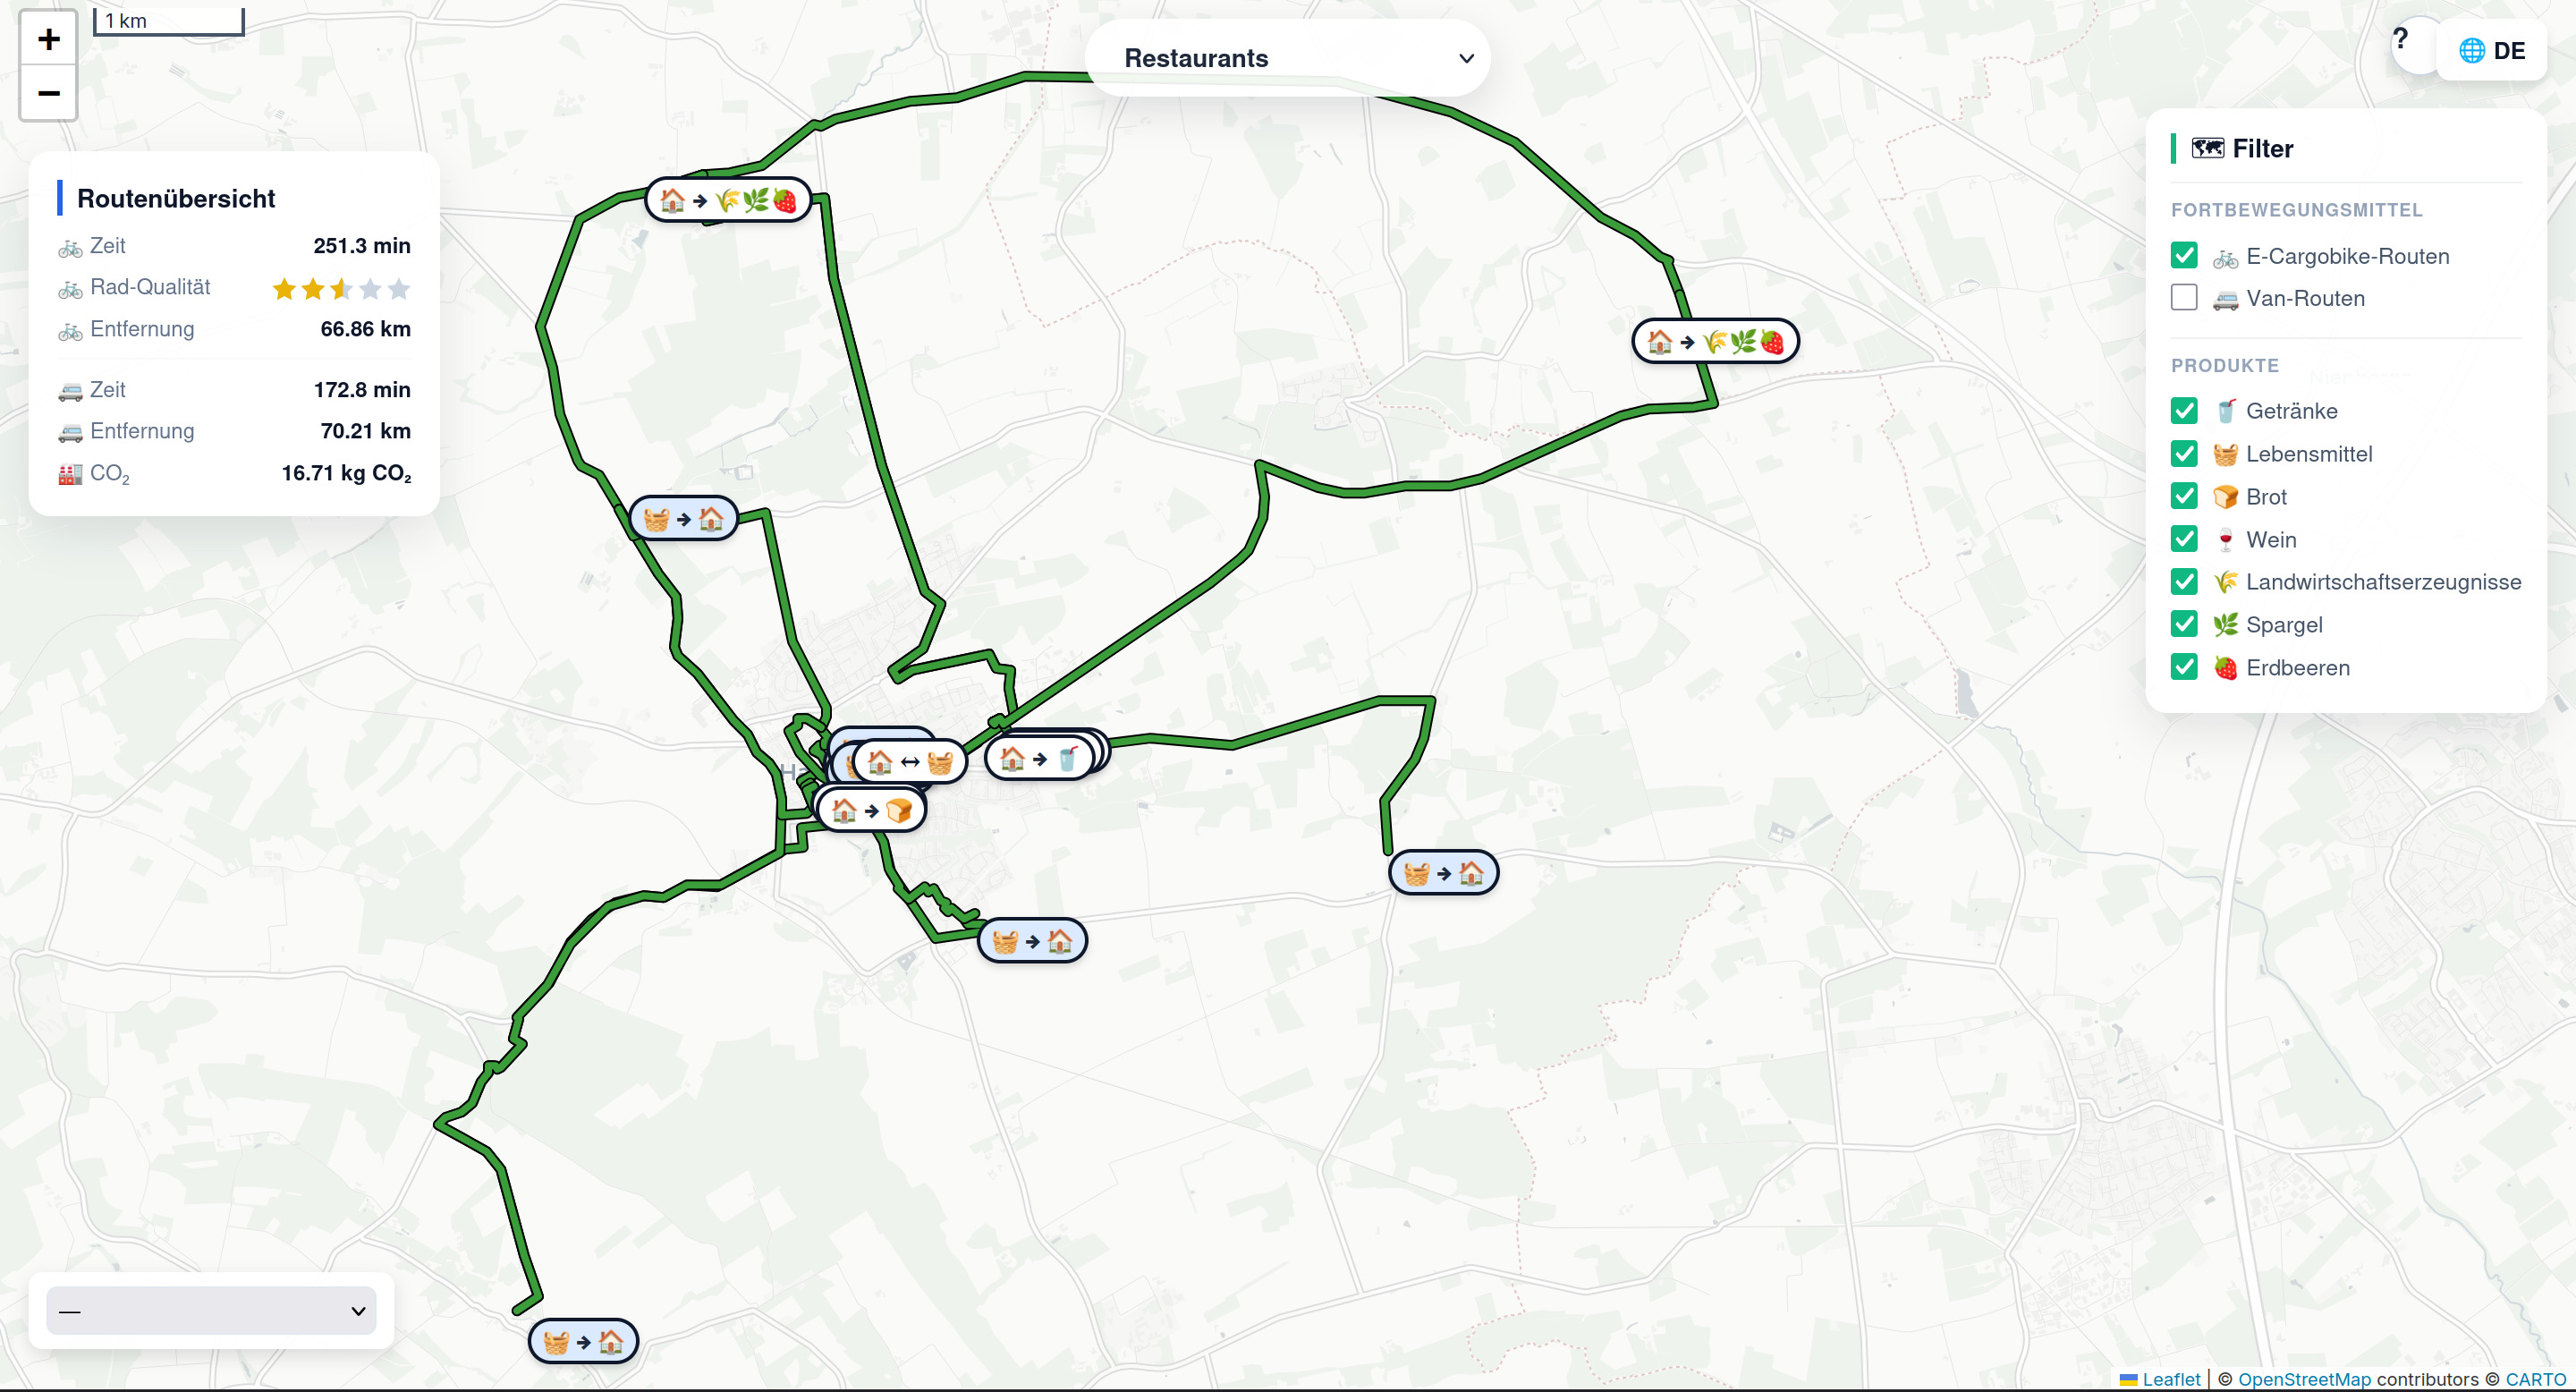
\includegraphics[width=0.85\textwidth]{figures/fig10_abholmodell_restaurants.jpg}
\caption[Abholmodell für Restaurants]{Variante mit einem Abholmodell für Restaurants (eigene Darstellung, Datenquelle: \cite{OpenStreetMap}\interaktivekarte[Restaurants][layer=custom_3])}
\label{fig:abholmodell}
\end{figure}

{\small
\begin{longtable}{@{}lrrrrrrr@{}}
\caption{Routen für das Abholkonzept}\label{tab:abholkonzept}\\
\toprule
\textbf{Standort} & \textbf{Pkw min} & \textbf{Pkw km} & \textbf{Pkw CO\textsubscript{2} kg} & \textbf{Rad min} & \textbf{Rad km} & \textbf{Mehrzeit \%} & \textbf{Score} \\
\midrule
\endfirsthead
\multicolumn{8}{@{}l}{\small\itshape Fortsetzung von der vorherigen Seite}\\
\toprule
\textbf{Standort} & \textbf{Pkw min} & \textbf{Pkw km} & \textbf{Pkw CO\textsubscript{2} kg} & \textbf{Rad min} & \textbf{Rad km} & \textbf{Mehrzeit \%} & \textbf{Score} \\
\midrule
\endhead
\midrule
\multicolumn{8}{@{}r}{\small\itshape Fortsetzung auf der nächsten Seite}\\
\endfoot
\bottomrule
\endlastfoot
Gasthaus Kemper   & 15,4  & 2,30  & 0,81  & 15,7  & 1,80  & 2,2  & 3,8 \\
Apollon           & 8,1   & 2,35  & 0,71  & 11,6  & 1,59  & 44,2 & 4,2 \\
Brauhaus Klute    & 23,5  & 8,30  & 2,43  & 34,3  & 8,65  & 46,1 & 8,1 \\
Haus Füsting      & 56,0  & 26,12 & 6,30  & 83,2  & 25,64 & 48,6 & 7,5 \\
Gasthaus Stevertal& 54,3  & 28,33 & 6,41  & 77,4  & 26,24 & 42,4 & 4,8 \\
Yosara            & 7,9   & 2,42  & 0,70  & 12,0  & 1,50  & 51,0 & 4,0 \\
Landg.\ Overwaul  & 18,7  & 9,40  & 1,92  & 29,4  & 9,40  & 57,7 & 3,0 \\
Wanjas            & 7,2   & 2,16  & 0,63  & 11,4  & 2,16  & 58,4 & 4,2 \\
\midrule
\textbf{Summe} & \textbf{191,0} & \textbf{81,39} & \textbf{19,92} & \textbf{275,0} & \textbf{76,98} & -- & -- \\
\textbf{Durchschnitt (Ø)} & -- & -- & -- & -- & -- & \textbf{43,8} & \textbf{5,0} \\
\end{longtable}
}

Bild~\ref{fig:abholmodell} und Tabelle~\ref{tab:abholkonzept} zeigen die berechneten Abholrouten. Wanjas, Apollon, Yosara und Gasthaus Kemper liegen zentrumsnah und eignen sich für ein Sharing-Lastenrad. Für Overwaul/Klute lohnt sich ein eigenes Rad, für Stevertal und Füsting bleibt der Pkw praktischer.

\subsection{Lebensmittelhandel (Anlieferung)}

\begin{figure}[htbp]
\centering
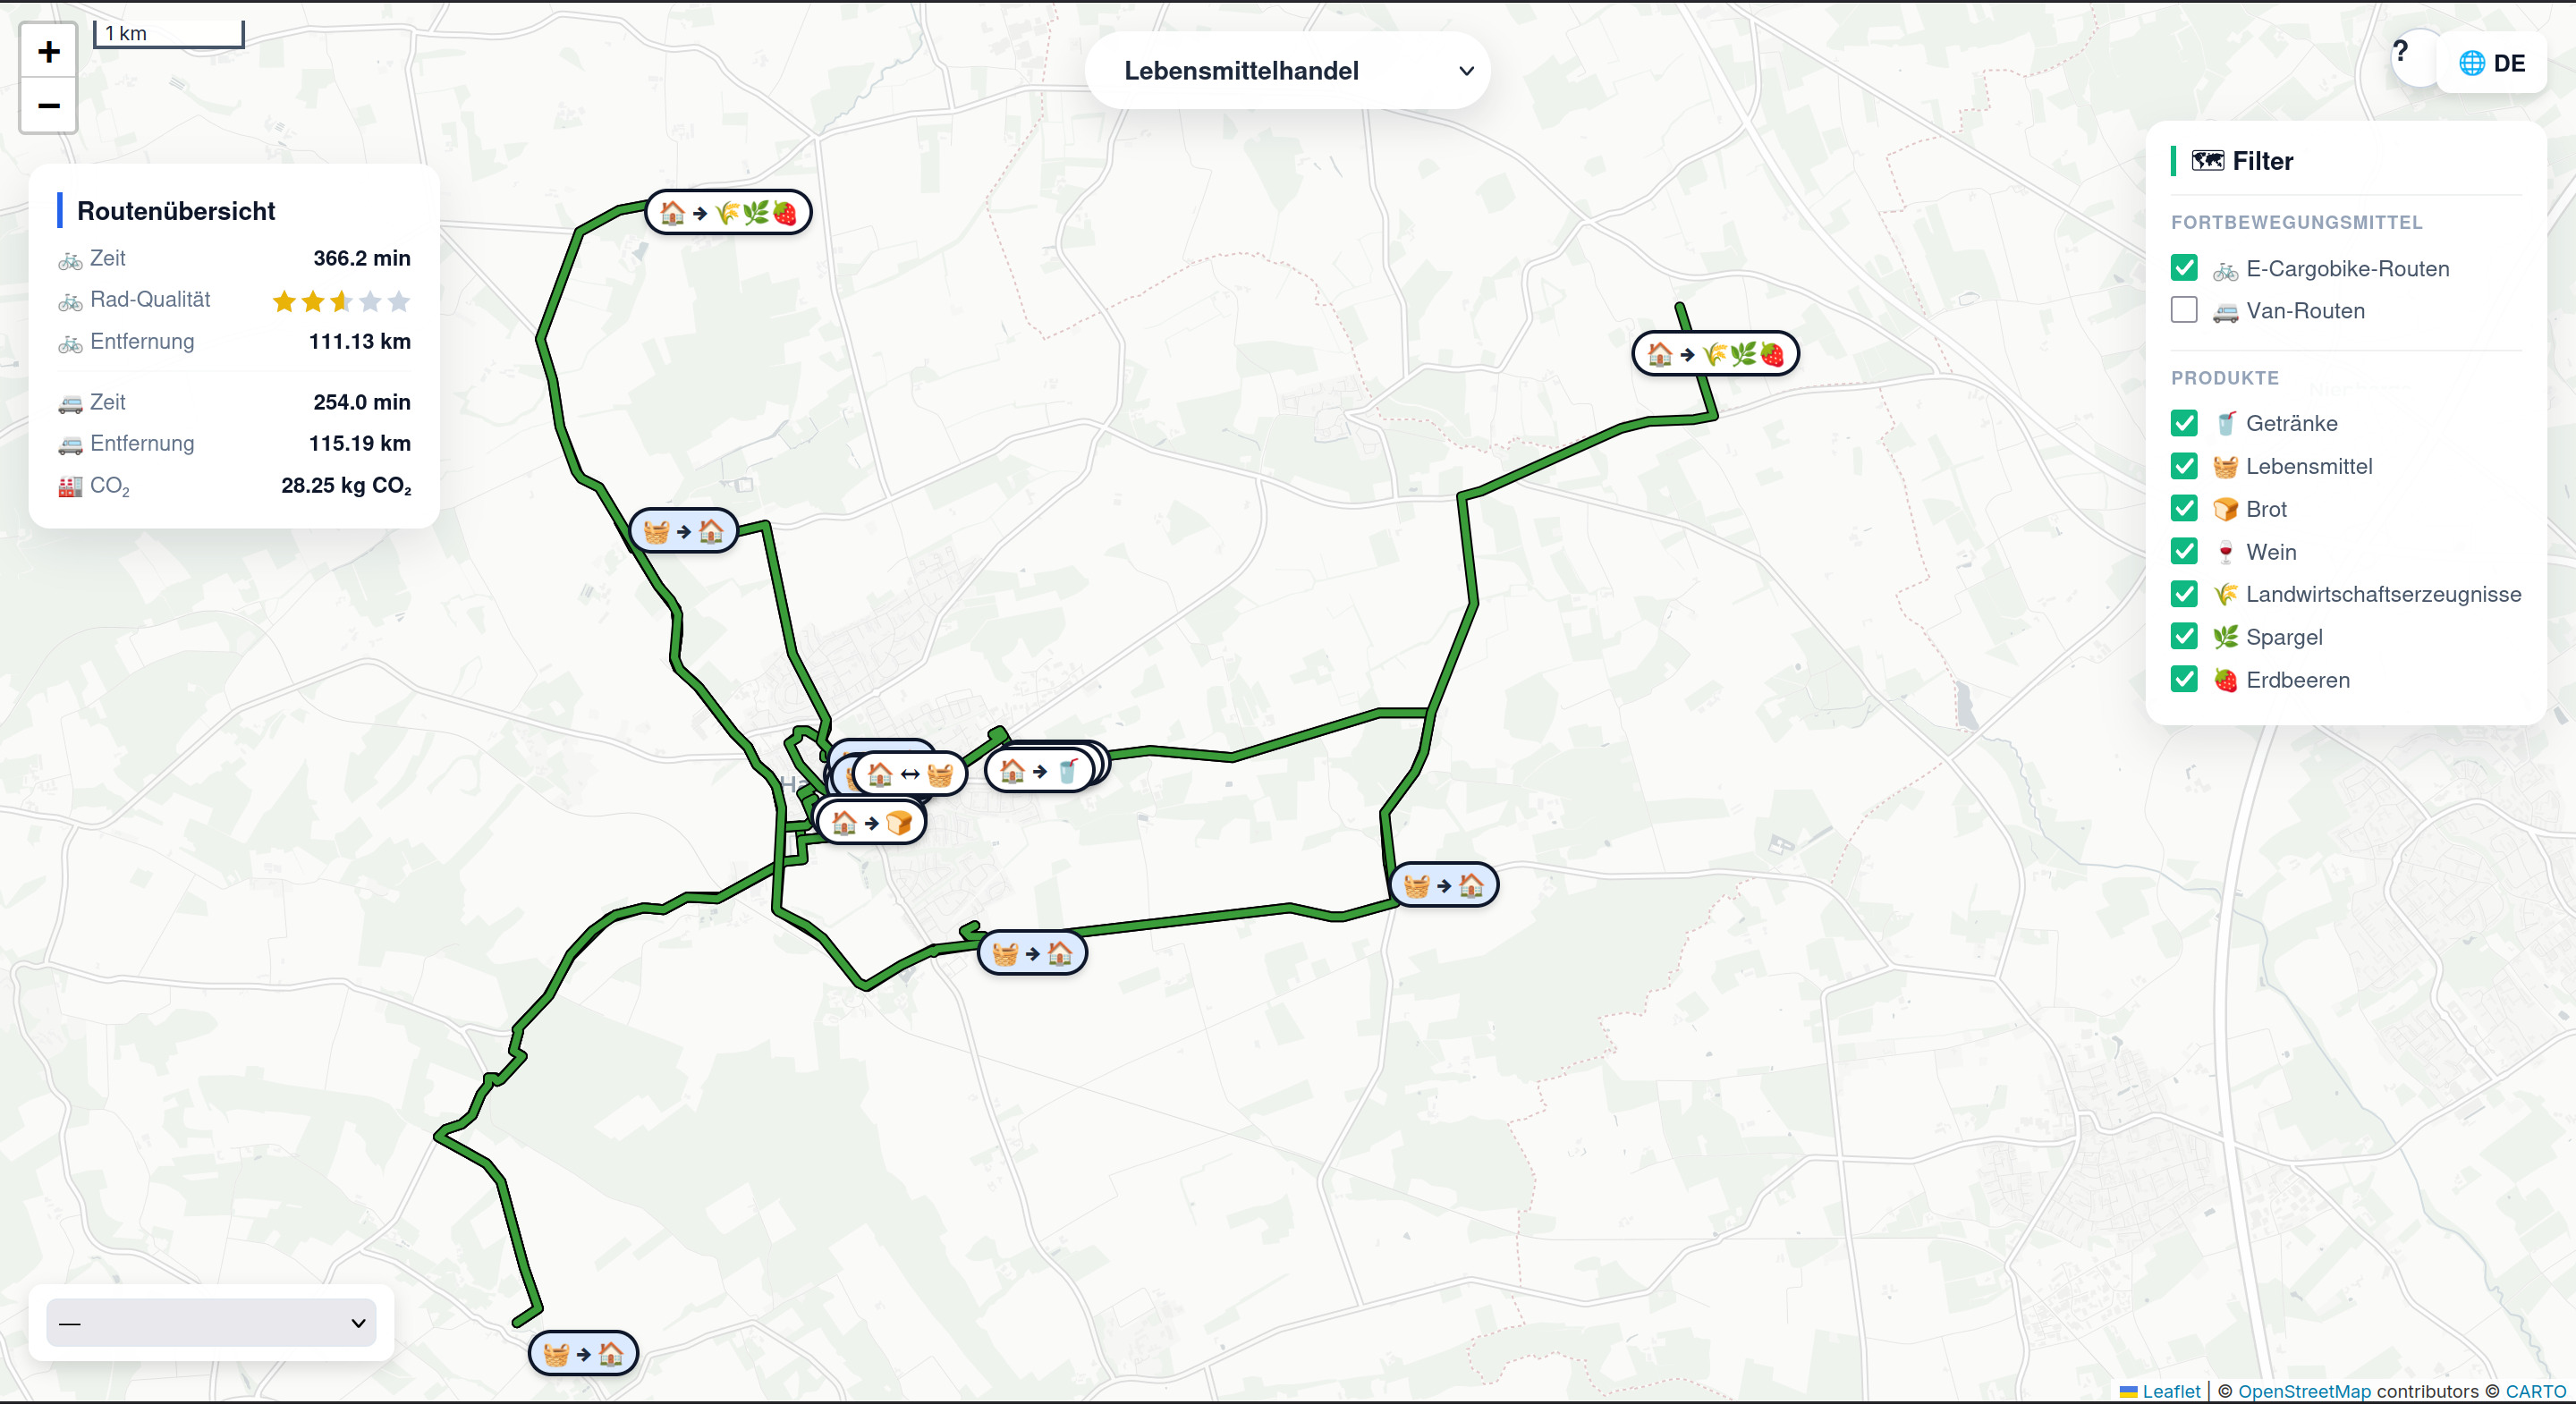
\includegraphics[width=0.85\textwidth]{figures/fig11_anliefermodell_restaurants.jpg}
\caption[Anliefermodell für Restaurants]{Variante mit einem Anliefermodell für Restaurants (eigene Darstellung, Datenquelle: \cite{OpenStreetMap}\interaktivekarte[Lebensmittelhandel][layer=custom_4])}
\label{fig:anliefermodell}
\end{figure}

{\small
\begin{longtable}{@{}lrrrrrrr@{}}
\caption{Routen für das Anlieferkonzept}\label{tab:anlieferkonzept}\\
\toprule
\textbf{Standort} & \textbf{Pkw min} & \textbf{Pkw km} & \textbf{Pkw CO\textsubscript{2} kg} & \textbf{Rad min} & \textbf{Rad km} & \textbf{Mehrzeit \%} & \textbf{Score} \\
\midrule
\endfirsthead
\multicolumn{8}{@{}l}{\small\itshape Fortsetzung von der vorherigen Seite}\\
\toprule
\textbf{Standort} & \textbf{Pkw min} & \textbf{Pkw km} & \textbf{Pkw CO\textsubscript{2} kg} & \textbf{Rad min} & \textbf{Rad km} & \textbf{Mehrzeit \%} & \textbf{Score} \\
\midrule
\endhead
\midrule
\multicolumn{8}{@{}r}{\small\itshape Fortsetzung auf der nächsten Seite}\\
\endfoot
\bottomrule
\endlastfoot
Wochenmarkt        & 8,2   & 0,33  & 0,19  & 4,0   & 0,33  & $-51,1$ & 3,1 \\
Trink \& Spare     & 19,1  & 7,64  & 2,20  & 26,9  & 8,02  & 40,6 & 8,9 \\
Der Weingarten     & 13,4  & 5,18  & 1,41  & 19,1  & 5,58  & 42,4 & 8,5 \\
Hof Heilers-Lülf   & 53,5  & 26,27 & 6,22  & 78,4  & 24,53 & 46,4 & 6,5 \\
Fröndhoff          & 45,8  & 23,11 & 5,39  & 67,2  & 21,37 & 46,7 & 4,4 \\
Netto              & 45,8  & 23,11 & 5,39  & 67,2  & 21,37 & 46,7 & 4,4 \\
Aldi               & 16,8  & 6,39  & 1,76  & 24,8  & 6,58  & 47,6 & 8,2 \\
Essmann            & 17,1  & 6,41  & 1,78  & 25,9  & 6,61  & 51,7 & 8,2 \\
Hof Baumeister     & 34,2  & 16,74 & 3,91  & 52,6  & 16,74 & 54,0 & 8,5 \\
\midrule
\textbf{Summe} & \textbf{254,0} & \textbf{115,19} & \textbf{28,25} & \textbf{366,2} & \textbf{111,13} & -- & -- \\
\textbf{Durchschnitt (Ø)} & -- & -- & -- & -- & -- & \textbf{36,1} & \textbf{6,7} \\
\end{longtable}
}

Bild~\ref{fig:anliefermodell} und Tabelle~\ref{tab:anlieferkonzept} zeigen die berechneten Lieferrouten. Geeignet fürs Lastenrad (auch Sharing): Der Weingarten, Aldi, Essmann, Trink \& Spare. Für ein eigenes Rad zusätzlich Fröndhoff, Netto und Hof Heilers-Lülf. Bei Hof Baumeister bleibt der Pkw besser.

\subsection{Abholung vs.\ Anlieferung}

{\small
\begin{longtable}{@{}lrr@{}}
\caption{Vergleich von Abhol- und Anlieferkonzepten}\label{tab:abhol-vs-anliefer}\\
\toprule
& \textbf{Restaurants holen ab} & \textbf{Handel liefert} \\
\midrule
\endfirsthead
\multicolumn{3}{@{}l}{\small\itshape Fortsetzung von der vorherigen Seite}\\
\toprule
& \textbf{Restaurants holen ab} & \textbf{Handel liefert} \\
\midrule
\endhead
\midrule
\multicolumn{3}{@{}r}{\small\itshape Fortsetzung auf der nächsten Seite}\\
\endfoot
\bottomrule
\endlastfoot
Anzahl Schleifen    & 8       & 10 \\
Pkw Distanz gesamt  & 70,2\,km  & 117,2\,km \\
Pkw Zeit gesamt     & 172,8\,min & 260,0\,min \\
Pkw CO\textsubscript{2} gesamt & 16,7\,kg & 28,3\,kg \\
Rad Distanz gesamt  & 66,9\,km  & 113,1\,km \\
Rad Zeit gesamt     & 251,3\,min & 376,2\,min \\
Ø Bike-Score        & 4,9     & 6,5 \\
\end{longtable}
}

Tabelle~\ref{tab:abhol-vs-anliefer} stellt beide Varianten gegenüber. Die Abholung ist distanz- und emissionsärmer, da Restaurants mehrere Lieferanten bündeln. Die Handelsrouten sind fahrradfreundlicher. Für die vier zentrumsnahen Restaurants ist Sharing naheliegend, sonst eher je ein eigenes Rad.

\chapter{Fazit und Ausblick}

Diese Arbeit ist von der Beobachtung ausgegangen, dass gerade im ländlichen Raum ein erheblicher Anteil kurzer Wege weiterhin mit dem Pkw zurückgelegt wird, obwohl Lastenräder hierfür grundsätzlich geeignet wären. Die Ist-Analyse der Logistikstrukturen in Havixbeck hat dieses Potenzial bestätigt, es jedoch klar branchen- und akteursabhängig eingegrenzt: Leichte, kleinteilige Güter mit kurzen Transportwegen eignen sich gut für die Verlagerung auf Lastenräder, schwere oder großvolumige Güter dagegen kaum. Auf dieser Grundlage wurden mit dem Stift Tilbeck sowie den landwirtschaftlichen Betrieben und Gastronomiebetrieben im Umland zwei Akteursgruppen mit besonders vielversprechenden Transportbeziehungen ausgewählt.

Die eigens entwickelte Routing-Engine hat es ermöglicht, für diese Akteure realistische Fahrzeiten, wahrgenommene Fahrzeiten und CO\textsubscript{2}-Bilanzen für Pkw und Lastenrad gegenüberzustellen. Sie zeigt: Auf kurzen, zentrumsnahen Strecken ist das Lastenrad zeitlich konkurrenzfähig oder sogar im Vorteil. Mit zunehmender Entfernung wächst die Mehrzeit gegenüber dem Pkw jedoch deutlich, und die reine Wegequalität, also getrennte Radwege, spielt gegenüber der Distanz eine untergeordnete Rolle. Die darauf aufbauende Auswertung der drei Konzepte in Kapitel~\ref{ch:massnahmen} bestätigt dieses Bild: Radlogistik kann den Pkw in Havixbeck nicht flächendeckend ersetzen. An mehreren klar identifizierten Stellen ist sie aber schon heute wirtschaftlich und ökologisch sinnvoll einsetzbar, etwa beim Stift Tilbeck, bei den zentrumsnahen Restaurants und am Wochenmarkt als gemeinsamem Treffpunkt.

Radlogistik lohnt sich vor allem bei kurzen Strecken, kleinen Mengen und guter Infrastruktur, etwa beim Stift Tilbeck oder den vier zentrumsnahen Restaurants. Bei Landwirtschaft und entfernterer Gastronomie entscheidet die Distanz, nicht die Wegqualität, da sehr viele Radwege vorhanden sind. Das Sharing-System lohnt sich nur für drei bis vier zentrale Restaurants und sollte auch für private Nutzung geöffnet werden.

Restaurants beziehen heute kaum lokale Produkte, sondern werden über Großhandel aus Münster versorgt. Radlogistik ersetzt das nicht, sondern ergibt nur Sinn, wenn parallel lokale Erzeugung gestärkt wird. Die ländliche Siedlungsstruktur macht eigene Mikro-Hubs meist überflüssig. Der Wochenmarkt erzielt aber einen ähnlichen Effekt, da dort Landwirtschaftsbetriebe und Restaurants ohnehin zusammenkommen. Außerdem eignet sich für Restaurants ein Abholsystem, bei dem die Waren direkt von landwirtschaftlichen Betrieben, dem Lebensmittelhandel oder dem Wochenmarkt bezogen werden, besser als ein Zubringersystem. Dadurch werden die Transportwege verkürzt und Fahrten gebündelt.

\section{Empfohlene Umsetzungsstufen}

\begin{itemize}
\item \textbf{Stift Tilbeck und Wochenmarkt-Pilot} fördern, denn diese Strecken sind schon heute die kürzesten und fahrradfreundlichsten.
\item \textbf{Sharing-System} für Wanjas, Apollon, Yosara und Gasthaus Kemper.
\item \textbf{Förderprogramm für lokalen Bezug}, damit Restaurants lokal erzeugte Produkte auch beziehen, sonst fehlt das Volumen.
\item \textbf{Anreize für Rad statt Pkw am Wochenmarkt}, etwa reservierte Lastenrad-Stellplätze oder eingeschränkter Pkw-Zugang am Markttag, sowie ein Förderprogramm oder bessere Rahmenbedingungen für Lastenrad-Verkaufsstand-Konstruktionen nach dem Vorbild von Stift Tilbeck.
\item \textbf{Ausweitung auf weitere Strecken}, sobald die meisten Betriebe einen Lastenrad-Anhänger für Wege wie zum Wochenmarkt besitzen: Mit Fahrzeug und Erfahrung vorhanden, lassen sich schrittweise auch andere wiederkehrende Strecken durch Radlogistik ersetzen.
\end{itemize}

\clearpage
\printbibliography[heading=bibintoc,title={Literaturverzeichnis}]

\end{document}
